%\documentclass[../main-physics-workbook.tex]{subfiles}

%...For a standalone document, un-comment lines below and recompile here:
\documentclass[]{exam}
\usepackage{marvosym}

%...TikZ & PGF
\usepackage{pgfplots}
\pgfplotsset{compat=1.11}
\tikzset{>=latex}
\usetikzlibrary{calc,math}
\usepackage{tikzsymbols}
\usepgfplotslibrary{fillbetween}
\usetikzlibrary{decorations.markings} 
\usetikzlibrary{arrows.meta} %...APP2 for arrows as objects and images
\usetikzlibrary{backgrounds} %...For shading portions of graphs
\usetikzlibrary{patterns} %...Unit 5 Problems
\usetikzlibrary{shapes.geometric} %...For drawing cylinders in Unit 2
\usepackage{makecell} %...use \thead{} to enable line skip in table headers
\tikzset{
    mark position/.style args={#1(#2)}{
        postaction={
            decorate,
            decoration={
                markings,
                mark=at position #1 with \coordinate (#2);
            }
        }
    }
} %...See https://tex.stackexchange.com/questions/43960/define-node-at-relative-coordinates-of-draw-plot

\tikzset{
    declare function = {trajectoryequation10(\x,\vi,\thetai)= tan(\thetai)*\x - 10*\x^2/(2*(\vi*cos(\thetai))^2);},
    declare function = {trajectoryequation(\x,\vi,\thetai)= tan(\thetai)*\x - 9.8*\x^2/(2*(\vi*cos(\thetai))^2);},
    declare function = {patheq(\x,\yi,\vi,\thetai)= \yi + tan(\thetai)*\x - 9.8*\x^2/(2*(\vi*cos(\thetai))^2);},
    declare function = {patheqten(\x,\yi,\vi,\thetai)= \yi + tan(\thetai)*\x - 10*\x^2/(2*(\vi*cos(\thetai))^2);} %like patheq but with gravity = 10
}

%...siunitx
\usepackage{siunitx}
\DeclareSIUnit{\nothing}{\relax}
\def\mymu{\SI{}{\micro\nothing} }
\DeclareSIUnit\mmHg{mmHg}
\DeclareSIUnit{\mile}{mi}
%...NOTE: "The product symbol between the number and unit is set using the quantity-product option."

%...Other
\usepackage{amsthm}
\usepackage{amsmath}
\usepackage{amssymb}
\usepackage{cancel}
\usepackage{subcaption}
\usepackage{dashrule}
\usepackage{enumitem}
\usepackage{fontawesome}
\usepackage{multicol}
\usepackage{glossaries}
%\numberwithin{equation}{section}
\numberwithin{figure}{section}
\usepackage{float}
\usepackage{twemojis} %...twitter emojis
\usepackage{utfsym}
\usepackage{linearb} %...For \BPwheel in Unit 8
\newcommand{\R}{\mathbb{R}} %...real number symbol
\usepackage{graphicx}
\graphicspath{ {../Figures/} }
\usepackage{hyperref}
\hypersetup{colorlinks=true,
    linkcolor=blue,
    filecolor=magenta,
    urlcolor=cyan,}
\urlstyle{same}
\newcommand{\hdashline}{{\hdashrule{\textwidth}{0.5pt}{0.8mm}}}
\newcommand{\hgraydashline}{{\color{lightgray} \hdashrule{0.99\textwidth}{1pt}{0.8mm}}}

%...Miscellaneous user-defined symbols
\newcommand{\fnet}{F_{\text{net}}} %...For net force
\newcommand{\bvec}[1]{\vec{\mathbf{#1}}} %...bold vector
\newcommand{\bhat}[1]{\,\hat{\mathbf{#1}}} %...bold hat vector
\newcommand{\que}{\mathord{?}}  %...Question mark symbol in equation env
%...Define thick horizontal rule for examples:
\newcommand{\hhrule}{\hrule\hrule}
\let\oldtexttt\texttt% Store \texttt
\renewcommand{\texttt}[2][black]{\textcolor{#1}{\ttfamily #2}}% 

%...For use in the exam document class
\newif\ifprintmetasolutions


%...Decreases space above and below align and gather enironment
\makeatletter
\g@addto@macro\normalsize{%
  \setlength\abovedisplayskip{-3pt}
  \setlength\belowdisplayskip{6pt} 
}
\makeatother





\usepackage[margin=1in]{geometry}
\usepackage[figurewithin=none]{caption}
\usepackage{exam-randomizechoices}
\setrandomizerseed{1}

\CorrectChoiceEmphasis{\color{red}\bfseries}
\renewcommand{\solutiontitle}{\noindent\textbf{\textcolor{red}{Solution:}}\enspace}

\usepackage{OutilsGeomTikz}
\usepackage{utfsym} %...Symbols in Unit 7 Problems
\usepackage{tabu} %...Symbols in Unit 7 Problems

%...For use in Unit 2            %    
\setlength{\columnsep}{2cm}      %
\setlength{\columnseprule}{1pt}  %
\usepackage[none]{hyphenat}      %
%%%%%%%%%%%%%%%%%%%%%%%%%%%%%%%%%

%...For use in Unit 11 on Waves:
\pgfdeclarehorizontalshading{visiblelight}{50bp}{  %
color(0.00000000000000bp)=(red);                   %
color(8.33333333333333bp)=(orange);                %
color(16.66666666666670bp)=(yellow);               %
color(25.00000000000000bp)=(green);                %
color(33.33333333333330bp)=(cyan);                 %
color(41.66666666666670bp)=(blue);                 %
color(50.00000000000000bp)=(violet)                %
}                                                  %

\newcommand{\checkbox}[1]{%
  \ifnum#1=1
    \makebox[0pt][l]{\raisebox{0.15ex}{\hspace{0.1em}\Large$\checkmark$}}%
  \fi
  $\square$%
}
%%%%%%%%%%%%%%%%%%%%%%%%%%%%%%%%%%%%%%%%%%%%%%%%%%%%

%...If using circuitikz package:
% \ctikzset{bipoles/battery1/height=0.5}
% \ctikzset{bipoles/battery1/width=0.25}
% \ctikzset{bipoles/resistor/height=0.15}
% \ctikzset{bipoles/resistor/width=0.4}
\makenoidxglossaries

%...UNIT 1: CONSTANT MOTION

\newglossaryentry{scalar}{
    name=scalar,
    description={a quantity that has magnitude (and possibly sign) but no direction}
}

\newglossaryentry{magnitude}{
    name={magnitude},
    description={size or amount}
}

\newglossaryentry{vector}{
    name={vector},
    description={a quantity that has both magnitude and direction}
}

\newglossaryentry{tail}{
    name={tail},
    description={the starting point of a vector; the point opposite to the head or tip of the arrow}
}

\newglossaryentry{head}{
    name={head},
    description={the end point of a vector; the location of the vector's arrow; also referred to as the tip}
}

\newglossaryentry{head-to-tail method}{
    name={head-to-tail method},
    description={a method of adding vectors in which the tail of each vector is placed at the head of the previous vector}
}

\newglossaryentry{position}{
    name={position},
    description={the location of an object at any particular time}
}

\newglossaryentry{reference frame}{
    name={reference frame},
    description={a coordinate system from which the positions of objects are described}
}


\newglossaryentry{displacement}{
    name={displacement},
    description={the change in position of an object against a fixed axis}
}

\newglossaryentry{distance}{
    name={distance},
    description={the length of the path actually traveled between an initial and a final position}
}

\newglossaryentry{position vs. time graph}{
    name={position vs. time graph},
    description={a graph in which position is plotted on the vertical axis and time is plotted on the horizontal axis}
}

\newglossaryentry{speed}{
    name={speed},
    description={rate at which an object changes its location}
}

\newglossaryentry{average speed}{
    name={average speed},
    description={distance traveled divided by the time during which the motion occurs}
}

\newglossaryentry{velocity}{
    name={velocity},
    description={the speed and direction of an object}
}

\newglossaryentry{average velocity}{
    name={average velocity},
    description={displacement divided by the time during which the displacement occurs}
}

\newglossaryentry{velocity vs. time graph}{
    name={velocity vs. time graph},
    description={a graph in which velocity is plotted on the vertical axis and time is plotted on the horizontal axis}
}

\newglossaryentry{mass}{
    name=mass,
    description={the quantity of matter in a substance; the SI unit of mass is the kilogram}
}

\newglossaryentry{inertia}{
    name=inertia,
    description={the tendency of an object at rest to remain at rest, or for a moving object to remain in motion in a straight line and at a constant speed}
}

\newglossaryentry{Newton's first law of motion}{
    name={Newton's first law of motion},
    description={a body at rest remains at rest or, if in motion, remains in motion at a constant speed in a straight line, unless acted on by a net external force; also known as the law of inertia}
}

\newglossaryentry{momentum}{
    name={momentum},
    description={the product of a system's mass and velocity}
}

\newglossaryentry{momentum vs. time graph}{
    name={momentum vs. time graph},
    description={a graph in which momentum is plotted on the vertical axis and time is plotted on the horizontal axis}
}

\newglossaryentry{kinetic energy}{
    name={kinetic energy},
    description={energy of motion}
}

\newglossaryentry{joule}{
    name=joule,
    description={the metric unit for work and energy; equal to 1 newton meter ($\text{N}\cdot\text{m}$)}
}

\newglossaryentry{relative speed}{
    name={relative speed},
    description={how fast or slow an object appears to be moving to another object}
}

\newglossaryentry{relative velocity}{
    name={relative velocity},
    description={the rate at which an object changes position relative to another object}
}

%...UNIT 2: FORCE INTERACTIONS

\newglossaryentry{force}{
    name=force,
    description={a push or pull on an object with a specific magnitude and direction; can be represented by vectors; can be expressed as a multiple of a standard force; the SI unit of force is the Newton (N)}
}

\newglossaryentry{external force}{
    name=external force,
    description={a force acting on an object or system that originates outside of the object or system}
}

\newglossaryentry{free body diagram}{
    name=free body diagram,
    description={a diagram showing all external forces acting on a body}
}

\newglossaryentry{frictional force}{
    name=frictional force,
    description={an external force that acts opposite to the direction of motion or, for when there is no relative motion, in the direction needed to prevent slipping}
}

\newglossaryentry{applied force}{
    name={applied force},
    description={a contact force intentionally implied by a person on an object}
}


\newglossaryentry{gravitational force}{
    name=gravitational force, %...MY DEFINITION
    description={the downward force on an object due to the attraction by the Earth or other massive body}
}

\newglossaryentry{net force}{
    name=net force,
    description={the sum of all forces acting on an object or system}
}

\newglossaryentry{normal force}{
    name=normal force,
    description={that component of the contact force between two objects, which acts perpendicularly to and away from their plane of contact}
}

\newglossaryentry{tension}{
    name=tension,
    description={a pulling force that acts along a connecting medium, especially a stretched flexible connector, such as a rope or cable; when a rope supports the weight of an object, the force exerted on the object by the rope is called tension}
}

\newglossaryentry{spring force}{
    name=spring force, %...From district slides
    description={a force applied from a spring when it is either compressed or stretched}
}

%...UNIT 3: ACCELERATION

\newglossaryentry{acceleration}{
    name={acceleration},
    description={a change in velocity over time}
}

\newglossaryentry{average acceleration}{
    name={average acceleration},
    description={change in velocity divided by the time interval over which it changed}
}

%...UNIT 4:


\newglossaryentry{impulse}{
    name={impulse},
    description={average net external force multiplied by the time the force acts; equal to the change in momentum}
}

\newglossaryentry{impulse-momentum theorem}{
    name={impulse-momentum theorem},
    description={the impulse equals change in momentum}
}

\newglossaryentry{work}{
    name={work},
    description={force multiplied by distance}
}

%...UNIT 5: FORCE ANALYSIS

\newglossaryentry{Newton's universal law of gravitation}{
    name={Newton's universal law of gravitation},
    description={states that gravitational force between two objects is directly proportional to the product of their masses and inversely proportional to the square of the distance between them}
}

\newglossaryentry{gravitational constant}{
    name={gravitational constant},
    description={the proportionality constant in Newton's law of universal gravitation}
}

\newglossaryentry{weight}{
    name={weight},
    description={the force of gravity, $W$, acting on an object of mass $m$; defined mathematically as $W = mg$, where $g$ is the acceleration due to gravity}
}

\newglossaryentry{contact force}{
    name={contact force},
    description={a type of force that occurs when objects are physically in contact with each other}
}

%...UNIT 6: ONE-DIMENSIONAL MOTION

\newglossaryentry{free fall}{
    name=free fall,
    description={a situation in which the only force acting on an object is the force of gravity}
}

\newglossaryentry{kinematic equations}{
    name={kinematic equations},
    description={the 
    %five 
    equations that describe constant acceleration motion in terms of time, displacement, velocity, and acceleration}
}

%...UNIT 7: MOTION IN TWO DIMENSIONS

\newglossaryentry{projectile}{
    name={projectile},
    description={an object that travels through the air and experiences only acceleration due to gravity}
}

\newglossaryentry{projectile motion}{
    name={projectile motion},
    description={the motion of an object that is subject only to the acceleration of gravity}
}

\newglossaryentry{trajectory}{
    name={trajectory},
    description={the path of a projectile through the air}
}

\newglossaryentry{apex}{
    name={apex},
    description={the location on the trajectory at which the projectile reaches maximum height}
}

\newglossaryentry{hang time}{
    name={hang time},
    description={the amount of time that a projectile is in the air during projectile motion}
}

\newglossaryentry{horizontally launched projectile}{
    name={horizontally launched projectile},
    description={a projectile whose initial velocity is entirely in the horizontal direction}
}

\newglossaryentry{impact speed}{
    name={impact speed},
    description={the speed at which a projectile strikes the ground after being launched}
}

%...UNIT 8: CONSERVATION IN MECHANICAL SYSTEMS

\newglossaryentry{system}{
    name={system},
    description={one or more objects of interest for which only the forces acting on them from the outside are considered, but not the forces acting between them or inside them}
}

\newglossaryentry{energy}{
    name={energy},
    description={the ability to do work}
}

\newglossaryentry{potential energy}{
    name={potential energy},
    description={stored energy}
}

\newglossaryentry{gravitational potential energy}{
    name={gravitational potential energy},
    description={energy acquired by doing work against gravity}
}

\newglossaryentry{law of conservation of energy}{
    name={law of conservation of energy},
    description={states that energy is neither created nor destroyed}
}

\newglossaryentry{mechanical energy}{
    name={mechanical energy},
    description={kinetic plus potential energy}
}

\newglossaryentry{elastic collision}{
    name={elastic collision},
    description={a collision in which objects separate after impact and kinetic energy is conserved}
}

\newglossaryentry{inelastic collision}{
    name={inelastic collision},
    description={a collision in which kinetic energy is not conserved}
}

\newglossaryentry{isolated system}{
    name={isolated system},
    description={system in which the net external force is zero}
}

\newglossaryentry{law of conservation of momentum}{
    name={law of conservation of momentum},
    description={when the net external force is zero, the total momentum of the system is conserved or constant}
}

\newglossaryentry{perfectly inelastic collision}{
    name={perfectly inelastic collision},
    description={collision in which objects stick together after impact and kinetic energy is not conserved}
}

\newglossaryentry{recoil}{
    name={recoil},
    description={backward movement of an object caused by the transfer of momentum from another object in a collision}
}

%...UNIT 9: CONSERVATION OF CHARGE

\newglossaryentry{electric charge}{
    name={electric charge},
    description={a physical property of an object that causes it to be attracted toward or repelled from another charged object; each charged object generates and is influenced by a force called an electromagnetic force}
}

\newglossaryentry{elementary charge}{
    name={elementary charge},
    description={the smallest observed unit of charge that can be isolated in nature; also, the magnitude of charge on 1 proton or 1 electron}
}

\newglossaryentry{electron}{
    name={electron},
    description={subatomic particle that carries one indivisible unit of negative electric charge}
}

\newglossaryentry{proton}{
    name={proton},
    description={subatomic particle that carries the same magnitude charge as the electron, but its charge is positive}
}

\newglossaryentry{electric field}{
    name={electric field},
    description={defines the force per unit charge at all locations in space around a charge distribution}
}

\newglossaryentry{law of conservation of charge}{
    name={law of conservation of charge},
    description={states that total charge is constant in any process}
}

\newglossaryentry{polarization}{
    name={polarization},
    description={separation of charge induced by nearby excess charge}
}

\newglossaryentry{Coulomb's law}{
    name={Coulomb's law},
    description={describes the electrostatic force between charged objects, which is proportional to the charge on each object and inversely proportional to the square of the distance between the objects}
}

\newglossaryentry{electric circuit}{
    name={electric circuit},
    description={physical network of paths through which electric current can flow}
}

\newglossaryentry{simple circuit}{
    name={simple circuit},
    description={a circuit with a single voltage source and a single resistor}
}

\newglossaryentry{electric current}{
    name={electric current},
    description={electric charge that is moving}
}


\newglossaryentry{Ohm's law}{
    name={Ohm's law},
    description={electric current is proportional to the voltage applied across a circuit or other path}
}

\newglossaryentry{resistance}{
    name={resistance},
    description={how much a circuit element opposes the passage of electric current; it appears as the constant of proportionality in Ohm’s law}
}

\newglossaryentry{resistor}{
    name={resistor},
    description={circuit element that provides a known resistance}
}

% \newglossaryentry{potential difference (or voltage)}{
%     name={potential difference (or voltage)},
%     description={change in potential energy of a charge moved from one point to another, divided by the charge; units of potential difference are joules per coulomb, known as volt}
% }

\newglossaryentry{voltage}{
    name={voltage},
    description={the electrical potential energy per unit charge; electric pressure created by a power source, such as a battery}
}

\newglossaryentry{electric power}{
    name={electric power},
    description={rate at which electric energy is transferred in a circuit}
}

\newglossaryentry{equivalent resistor}{
    name={equivalent resistor},
    description={resistance of a single resistor that is the same as the combined resistance of a group of resistors}
}

\newglossaryentry{in series}{
    name={in series},
    description={when elements in a circuit are connected one after the other in the same branch of the circuit}
}

\newglossaryentry{in parallel}{
    name={in parallel},
    description={when a group of resistors are connected side by side, with the top ends of the resistors connected together by a wire and the bottom ends connected together by a different wire}
}

\newglossaryentry{induction}{
    name={induction},
    description={creating an unbalanced charge distribution in an object by moving a charged object toward it (but without touching)}
}

%...UNIT 10: ELECTROMAGNETIC INDUCTION

\newglossaryentry{magnetic dipole}{
    name={magnetic dipole},
    description={term that describes magnets because they always have two poles: north and south}
}

\newglossaryentry{magnetic field}{
    name={magnetic field},
    description={directional lines around a magnetic material that indicates the direction and magnitude of the magnetic force}
}

\newglossaryentry{magnetic pole}{
    name={magnetic pole},
    description={part of a magnet that exerts the strongest force on other magnets or magnetic material}
}

\newglossaryentry{electromagnetic induction}{
    name={electromagnetic induction},
    description={rate at which energy is drawn from a source per unit current flowing through a circuit}
}


\newglossaryentry{Faraday's law}{
    name={Faraday's law},
    description={the means of calculating the emf in a coil due to changing magnetic flux}
}

\newglossaryentry{electromagnet}{
    name={electromagnet},
    description={device that uses electric current to make a magnetic field}
}

\newglossaryentry{transformer}{
    name={transformer},
    description={device that transforms voltages from one value to another}
}

\newglossaryentry{electric motor}{
    name={electric motor},
    description={device that transforms electrical energy into mechanical energy}
}

\newglossaryentry{generator}{
    name={generator},
    description={device that transforms mechanical energy into electrical energy}
}

%...UNIT 11: SIMPLE HARMONIC MOTION & WAVES

\newglossaryentry{wave}{
    name={wave},
    description={a disturbance that moves from its source and carries energy}
}

\newglossaryentry{wave velocity}{
    name={wave velocity},
    description={speed at which the disturbance moves; also called the propagation velocity or propagation speed}
}

\newglossaryentry{wavelength}{
    name={wavelength},
    description={distance between adjacent identical parts of a wave}
}

\newglossaryentry{wave cycle}{
    name={wave cycle},
    description={any portion of a wave encompassed by 1 wavelength}
}

\newglossaryentry{transverse wave}{
    name={transverse wave},
    description={a wave in which the disturbance is perpendicular to the direction of propagation}
}

\newglossaryentry{medium}{
    name={medium},
    description={the solid, liquid, or gas material through which a wave propagates}
}

\newglossaryentry{mechanical wave}{
    name={mechanical wave},
    description={wave that requires a medium through which it can travel}
}

\newglossaryentry{longitudinal wave}{
    name={longitudinal wave},
    description={wave in which the disturbance is parallel to the direction of propagation}
}

\newglossaryentry{constructive interference}{
    name={constructive interference},
    description={when two waves arrive at the same point exactly in phase; that is, the crests of the two waves are precisely aligned, as are the troughs}
}

\newglossaryentry{destructive interference}{
    name={destructive interference},
    description={when two identical waves arrive at the same point exactly out of phase that is precisely aligned crest to trough}
}

\newglossaryentry{oscillate}{
    name={oscillate},
    description={to move back and forth regularly between two points}
}

\newglossaryentry{amplitude}{
    name={amplitude},
    description={the maximum displacement from the equilibrium position of an object oscillating around the equilibrium position}
}

\newglossaryentry{frequency}{
    name={frequency},
    description={number of wave cycles per unit of time}
}

\newglossaryentry{simple harmonic motion}{
    name={simple harmonic motion},
    description={the oscillatory motion in a system where the net force can be described by Hooke’s law}
}

\newglossaryentry{simple harmonic oscillator}{
    name={simple harmonic oscillator},
    description={a device that oscillates in SHM,  such as a mass that is attached to a spring, where the restoring force is proportional to the displacement and acts in the direction opposite to the displacement}
}

\newglossaryentry{period}{
    name={period},
    description={the time it takes to complete one oscillation}
}

\newglossaryentry{electromagnetic wave}{
    name={electromagnetic wave},
    description={a radiant energy wave that consists of oscillating electric and magnetic fields}
}

\newglossaryentry{electromagnetic radiation}{
    name={electromagnetic radiation},
    description={radiant energy that consists of oscillating electric and magnetic fields}
}









%... Overview and Student Learning Expectations (OSLE)

\newglossaryentry{OSLE 6.1.a}{
    name={OSLE 6.1.a},
    description={compare the gravitational field strength on Earth to the acceleration due to gravity on Earth}
}

\newglossaryentry{OSLE 6.1.b}{
    name={OSLE 6.1.b},
    description={explain using universal gravitation and $F_\mathrm{net}=ma$ why all objects near Earth's surface fall at the same rate when in free fall}
}

\newglossaryentry{OSLE 6.1.c}{
    name={OSLE 6.1.c},
    description={explain the relationship between the mass, initial position, and initial velocity of an object in free fall on its final velocity and/or time in free fall}
}

\newglossaryentry{OSLE 6.1.d}{
    name={OSLE 6.1.d},
    description={describe the displacement, velocity, momentum, kinetic energy, and acceleration of an object in free fall that was dropped, thrown upward, or thrown downward using Multiple Representations}
}

\newglossaryentry{OSLE 6.1.e}{
    name={OSLE 6.1.e},
    description={relate the gravitational force, impulse, and work done on the object by the Earth to the object's change in velocity (acceleration), momentum, and kinetic energy}
}

        
\newglossaryentry{OSLE 6.2.a}{
    name={OSLE 6.2.a},
    description={describe what is known about an object's motion in a constant acceleration word problem using Multiple Representations}
}

\newglossaryentry{OSLE 6.2.b}{
    name={OSLE 6.2.b},
    description={solve for various unknown quantities utilizing kinematic equations when data is given in Multiple Representations for objects moving horizontally with constant acceleration}
}

\newglossaryentry{OSLE 6.3.c}{
    name={OSLE 6.3.c},
    description={solve for various unknown quantities utilizing kinematic equations when data is given in Multiple Representations for objects moving vertically with constant acceleration (free fall)}
}

\newglossaryentry{OSLE 6.4.d}{
    name={OSLE 6.4.d},
    description={solve multi-step problems that connect kinematic equations, the Law of Acceleration, Work-Energy Theorem, and/or the Impulse-Momentum Theorem}
}

\newglossaryentry{OSLE 7.1.a}{
    name={OSLE 7.1.a},
    description={compare the trajectory, hang time, max height, range, and final velocity of various projectiles that have different initial velocities, launch heights, launch angles, and masses, only varying one parameter at a time}
}

\newglossaryentry{OSLE 7.1.b}{
    name={OSLE 7.1.b},
    description={identify if and explain how the  initial velocity, launch height, launch angle, and mass of a projectile influence its motion---hang time, height, range, final velocity}
}

\newglossaryentry{OSLE 7.2.a}{
    name={OSLE 7.2.a},
    description={describe the vertical and horizontal motion of a projectile with a launch angle of zero using Multiple Representations}
}

\newglossaryentry{OSLE 7.2.b}{
    name={OSLE 7.2.b},
    description={illustrate the resultant motion of the projectile at any point in its trajectory as well as the relationship between the horizontal and vertical components using vector addition}
}

\newglossaryentry{OSLE 7.2.c}{
    name={OSLE 7.2.c},
    description={analyze and solve word problems about the motion of  horizontally launched projectiles using kinematic equations, vector addition, and  Multiple Representations}
}

\newglossaryentry{OSLE 7.3.a}{
    name={OSLE 7.3.a},
    description={describe the motion of an object moving with uniform circular motion in terms of centripetal force, centripetal acceleration, momentum, kinetic energy, and tangential velocity using Multiple Representations}
}

\newglossaryentry{OSLE 7.3.b}{
    name={OSLE 7.3.b},
    description={determine the centripetal force, mass, centripetal acceleration, tangential velocity, or radius of an object in circular motion}
}

\newglossaryentry{OSLE 7.4.a}{
    name={OSLE 7.4.a},
    description={predict the effects of changing the radius or mass of objects in orbiting systems using concepts of uniform circular motion and Newton’s law of universal gravitation}
}


\newglossaryentry{OSLE 8.1.a}{
    name={OSLE 8.1.a},
    description={identify multiple choices for a system given a scenario}
}

\newglossaryentry{OSLE 8.1.b}{
    name={OSLE 8.1.b},
    description={recognize that energy can be stored in the arrangement of particles or objects in a system as potential energy}
}

\newglossaryentry{OSLE 8.1.c}{
    name={OSLE 8.1.c},
    description={identify and calculate (i) gravitational potential energy and (ii) elastic potential energy when a system includes energy stored in the arrangement of its particles or objects}
}

\newglossaryentry{OSLE 8.1.d}{
    name={OSLE 8.1.d},
    description={compare the potential energy of a scenario for various choices of system}
}

\newglossaryentry{OSLE 8.1.e}{
    name={OSLE 8.1.e},
    description={identify, represent using multiple representations, and calculate the total mechanical energy present in a physical system}
}

\newglossaryentry{OSLE 8.1.f}{
    name={OSLE 8.1.f},
    description={predict the effects of changing the mass, velocity, height, gravitational field strength, spring constant, compression or stretching distance on the amount of $E_k$, $E_\mathrm{GP}$, and $E_\mathrm{SP}$}
}

\newglossaryentry{OSLE 8.1.g}{
    name={OSLE 8.1.g},
    description={calculate the total mechanical energy of a system}
}

\newglossaryentry{OSLE 8.2.a.i}{
    name={OSLE 8.2.a.i},
    description={identify, represent using multiple representations, and calculate the amount of energy (1) transformed from one storage mode to another within a system (including kinetic energy, potential energy, and thermal energy), (2) transferred from one object in the system to another in the system, and (3) entering/leaving a system due to work, heat, light, or sound}
}

\newglossaryentry{OSLE 8.2.b.i}{
    name={OSLE 8.2.b.i},
    description={explain the meaning of the Law of Conservation of Energy}
}

\newglossaryentry{OSLE 8.2.b.ii}{
    name={OSLE 8.2.b.ii},
    description={develop an energy formula for systems using energy bar charts and the Law of Conservation of Energy}
}

\newglossaryentry{OSLE 8.2.b.iii}{
    name={OSLE 8.2.b.iii},
    description=solve for various unknown quantities using the concept of the conservation of energy{}
}

\newglossaryentry{OSLE 8.2.c.i}{
    name={OSLE 8.2.c.i},
    description={know the definition of work as change in energy of a system}
}

\newglossaryentry{OSLE 8.2.c.ii}{
    name={OSLE 8.2.c.ii},
    description={know that power is work done divided by time}
}

\newglossaryentry{OSLE 8.3.a}{
    name={OSLE 8.3.a},
    description={calculate and compare the momentum, changes in momentum, force applied to and impulse on each object involved in a collision or explosion scenario}
}

\newglossaryentry{OSLE 8.3.b}{
    name={OSLE 8.3.b},
    description={represent using multiple representations, compare, and calculate the total momentum of a system before and after a collision or explosion scenario}
}

\newglossaryentry{OSLE 8.3.c}{
    name={OSLE 8.3.c},
    description={explain the meaning of the Law of Conservation of Momentum}
}

\newglossaryentry{OSLE 8.3.d}{
    name={OSLE 8.3.d},
    description={solve for unknown quantities using the concept of the conservation of momentum}
}


\newglossaryentry{OSLE 9.1.a}{
    name={OSLE 9.1.a},
    description={identify the particles that contribute positive, negative, or no charge in an atom}
}

\newglossaryentry{OSLE 9.1.b}{
    name={OSLE 9.1.b},
    description={recognize that neutral objects have even numbers of positive and negative charges}
}

\newglossaryentry{OSLE 9.1.c}{
    name={OSLE 9.1.c},
    description={determine the charge of an object given the number of protons and electrons}
}

\newglossaryentry{OSLE 9.1.d}{
    name={OSLE 9.1.d},
    description={predict if two objects will attract, repel, or have no interaction based on their charges}
}

\newglossaryentry{OSLE 9.1.e}{
    name={OSLE 9.1.e},
    description={draw the electric field surrounding single charges and pairs of charges}
}

\newglossaryentry{OSLE 9.2.a}{
    name={OSLE 9.2.a},
    description={recognize that charge is conserved: it cannot be created or destroyed, only transferred}
}

\newglossaryentry{OSLE 9.2.b}{
    name={OSLE 9.2.b},
    description={realize that only electrons are transferred during charging}
}

\newglossaryentry{OSLE 9.2.c}{
    name={OSLE 9.2.c},
    description={compare and contrast charging by induction and conduction}
}

\newglossaryentry{OSLE 9.2.d}{
    name={OSLE 9.2.d},
    description={explain how polarization temporarily charges a neutral object}
}

\newglossaryentry{OSLE 9.2.e}{
    name={OSLE 9.2.e},
    description={describe how an electroscope determines if objects are charged}
}

\newglossaryentry{OSLE 9.2.f}{
    name={OSLE 9.2.f},
    description={determine whether an object is negatively charged, positively charged, or neutral when given the charge of one object and a description or diagram representing how the charged object interacts with an object of unknown charge}
}

\newglossaryentry{OSLE 9.2.g}{
    name={OSLE 9.2.g},
    description={draw and describe the resulting distribution of charge for various scenarios of induction, conduction, and polarization}
}


\newglossaryentry{OSLE 9.3.a}{
    name={OSLE 9.3.a},
    description={draw the free body diagram for 2 charged objects showing the direction and relative magnitude of the electrical force acting on each object at various distances from each other}
}

\newglossaryentry{OSLE 9.3.b}{
    name={OSLE 9.3.b},
    description={describe how the electric force depends on the charges and the distance between them}
}

\newglossaryentry{OSLE 9.3.c}{
    name={OSLE 9.3.c},
    description={compare and contrast the electric force to the gravitational force}
}

\newglossaryentry{OSLE 9.3.d}{
    name={OSLE 9.3.d},
    description={predict how changing the charge or distance affects the electric force}
}


\newglossaryentry{OSLE 9.4.a}{
    name={OSLE 9.4.a},
    description={identify the necessary components for a simple circuit and discover different ways to light a bulb}
}

\newglossaryentry{OSLE 9.4.b}{
    name={OSLE 9.4.b},
    description={trace the conducting path through a simple circuit}
}

\newglossaryentry{OSLE 9.4.c}{
    name={OSLE 9.4.c},
    description={explain the concepts of current, resistance, voltage}
}

\newglossaryentry{OSLE 9.4.d}{
    name={OSLE 9.4.d},
    description={measure the current, resistance and voltage in a circuit using a multimeter, ammeter, current probe, etc}
}

\newglossaryentry{OSLE 9.4.e}{
    name={OSLE 9.4.e},
    description={calculate the voltage drop across, current through, or resistance of a circuit component using Ohm’s Law}
}

\newglossaryentry{OSLE 9.4.f}{
    name={OSLE 9.4.f},
    description={determine the change in current as the voltage or resistance is changed}
}

\newglossaryentry{OSLE 9.4.g}{
    name={OSLE 9.4.g},
    description={interpret electrical power as the rate at which electrical energy is being dissipated in the circuit}
}

\newglossaryentry{OSLE 9.4.h}{
    name={OSLE 9.4.h},
    description={relate the power rating/wattage of a light bulb to its brightness}
}


\newglossaryentry{OSLE 9.5.a}{
    name={OSLE 9.5.a},
    description={measure the current, resistance and voltage at various locations in a series circuit using a multimeter, ammeter, current probe, etc}
}

\newglossaryentry{OSLE 9.5.b}{
    name={OSLE 9.5.b},
    description={describe qualitatively and quantitatively the current flow throughout a series circuit}
}

\newglossaryentry{OSLE 9.5.c}{
    name={OSLE 9.5.c},
    description={calculate the equivalent resistance of multiple resistors in series}
}

\newglossaryentry{OSLE 9.5.d}{
    name={OSLE 9.5.d},
    description={calculate the equivalent voltage of batteries in series}
}

\newglossaryentry{OSLE 9.5.e}{
    name={OSLE 9.5.e},
    description={recognize that the sum of the voltage drops across resistors in series equals the total voltage of the power supply}
}

\newglossaryentry{OSLE 9.5.f}{
    name={OSLE 9.5.f},
    description={describe the energy transformations (transfers) occurring in a series circuit}
}

\newglossaryentry{OSLE 9.5.g}{
    name={OSLE 9.5.g},
    description={determine (i) current through, voltage drop across, and power of each component, and (i) total current of circuit, when given a series circuit diagram}
}


\newglossaryentry{OSLE 9.6.a}{
    name={OSLE 9.6.a},
    description={measure the current, resistance and voltage at various locations in a parallel circuit using a multimeter, ammeter, current probe, etc}
}

\newglossaryentry{OSLE 9.6.b}{
    name={OSLE 9.6.b},
    description={recognize that the current going into a junction is equal to the current coming out of it}
}

\newglossaryentry{OSLE 9.6.c}{
    name={OSLE 9.6.c},
    description={describe qualitatively and quantitatively the current flow throughout a parallel circuit}
}

\newglossaryentry{OSLE 9.6.d}{
    name={OSLE 9.6.d},
    description={recognize that the voltage drops across each resistor are equal to the voltage of the power supply}
}

\newglossaryentry{OSLE 9.6.e}{
    name={OSLE 9.6.e},
    description={describe advantages and disadvantages of parallel circuits compared to series circuits}
}

\newglossaryentry{OSLE 9.6.f}{
    name={OSLE 9.6.f},
    description={calculate the equivalent resistance of multiple resistors in parallel}
}

\newglossaryentry{OSLE 9.6.g}{
    name={OSLE 9.6.g},
    description={calculate the equivalent voltage of batteries in parallel}
}

\newglossaryentry{OSLE 9.6.h}{
    name={OSLE 9.6.h},
    description={describe the energy transformations (transfers) occurring in a parallel circuit}
}

\newglossaryentry{OSLE 9.6.i}{
    name={OSLE 9.6.i},
    description={determine the (i) current through, voltage drop across, and power of each component, and (ii) total current of circuit, when given a series circuit diagram}
}


\newglossaryentry{OSLE 9.7.a}{
    name={OSLE 9.7.a},
    description={determine whether elements of a combination circuit have the same current or voltage}
}

\newglossaryentry{OSLE 9.7.b}{
    name={OSLE 9.7.b},
    description={predict which bulbs will light if switches are open or closed}
}







\setcounter{section}{9}
\usepackage{circuitikz}
\ctikzset{bipoles/battery1/height=0.5}
\ctikzset{bipoles/battery1/width=0.25}
\ctikzset{bipoles/resistor/height=0.15}
\ctikzset{bipoles/resistor/width=0.4}
\ctikzset{bipoles/cuteswitch/thickness=0.3,bipoles/cuteswitch/shape=circ}
\ctikzset{bipoles/bulb/height=0.4,bipoles/bulb/width=0.4}
\usepackage{bohr}

\header{Name:\enspace\makebox[5cm]{\hrulefill}}{}{}

\begin{document}



\textbf{\Large Charges and Matter}

\subsection{The Millikan's Oil Drop Experiment}

\textbf{Questions \ref{6YGfUm}--\ref{Q68N4Y}.} Watch ``Charge of an Electron: Millikan's Oil Drop Experiment'' by Tyler DeWitt on YouTube (\href{https://youtu.be/2HhaQtvICe8}{click here}), then answer the exercises below.

\begin{questions}
\question \label{6YGfUm}
In what year did Millikan and Fletcher conduct the oil drop experiment?


\question
J.~J.~Thompson discovered the electron, the negatively charged particle, in the year \rule{2cm}{0.15mm}.


\question
The Millikan's oil drop experiment involves balancing tiny drops of oil by using gravity and \rule{2cm}{0.15mm}.



\question
Two parts of the equipment used by Millikan are the \rule{2cm}{0.15mm} and the \rule{2cm}{0.15mm}.


\question
Which force acts downward on the oil drop?


\question
Which plate--the positively or the negatively charged---will the positive oil drop be attracted to? Explain.


\question
What force pushes the oil drop in the opposite direction of gravity?


\question
When the voltage is too HIGH, the oil drop moves \rule{2cm}{0.15mm}.


\question
When the voltage is too LOW, the oil drop moves \rule{2cm}{0.15mm}.


\question
What happens to the oil drop when the voltage through the apparatus is just right?


\question
The force of gravity on the drop depends only on the \rule{2cm}{0.15mm} of the drop.


\question
What 2 factors does the force of electricity on the drop depend on?


\question \label{Q68N4Y}
What is the charge of 1 electron?

\end{questions}



\clearpage
\subsection{The Electric Field}

\begin{questions}

\question
Go to the \href{https://phet.colorado.edu/sims/html/charges-and-fields/latest/charges-and-fields_all.html}{PhET Simulation: Charges and Fields}. Check only the following boxes: \checkbox{1} Electric Field, \checkbox{1}~Voltage, \checkbox{1} Grid. In this simulation, you may place charges onto the provided grid. The yellow sensor, when placed at any location, measures the magnitude (size) and direction of the electric field due to one or more charges.

\begin{parts}
\part In the PhET Simulation, place a positive charge aligned with the center of the grid. Then place sensors at each of the points shown in the grid below. \textbf{NOTE:} Place all items \textit{exactly} on the grid line intersections as shown. Then use the space below to draw the electric field vectors exactly to scale as shown in the simulation. Finally, repeat these steps for a single negative charge.

\begin{EnvUplevel}
\begin{center}
\begin{tikzpicture}
    \draw (-4,-4) grid (4,4);
    \draw[step=0.2,ultra thin,black!20] (-4,-4) grid (4,4);
    \draw[thick] (-4,-4) rectangle (4,4);
    \fill[white] (0,0) circle (0.2cm);
    \node at (0,0) {\resizebox{0.4cm}{!}{\faPlusCircle}};

    \ifprintanswers
    \bgroup
    \color{red}
    \draw[ultra thick,->] (-2,+2) -- ++(-0.75,+0.75);
    \draw[ultra thick,->] (-2.4,0) -- ++(-1.5,0);
    \draw[ultra thick,->] (-2,-2) -- ++(-0.75,-0.75);
    \draw[ultra thick,->] (0,-2.4) -- ++(0,-1.5);
    \draw[ultra thick,->] (+2,-2) -- ++(+0.75,-0.75);
    \draw[ultra thick,->] (+2.4,0) -- ++(+1.5,0);
    \draw[ultra thick,->] (+2,+2) -- ++(+0.75,+0.75);
    \draw[ultra thick,->] (0,+2.4) -- ++(0,+1.5);
    \egroup
    \fi

    \fill (-2,+2) circle (3pt);
    \fill (-2.4,0) circle (3pt);
    \fill (-2,-2) circle (3pt);
    \fill (0,-2.4) circle (3pt);
    \fill (+2,-2) circle (3pt);
    \fill (+2.4,0) circle (3pt);
    \fill (+2,+2) circle (3pt);
    \fill (0,+2.4) circle (3pt);
    \draw[ultra thick,<->] (-3,-4) -- (-1,-4) node[above,pos=0.5] {1 meter};
\end{tikzpicture}
\hspace{2mm}
\begin{tikzpicture}
    \draw (-4,-4) grid (4,4);
    \draw[step=0.2,ultra thin,black!20] (-4,-4) grid (4,4);
    \draw[thick] (-4,-4) rectangle (4,4);
    \fill[white] (0,0) circle (0.2cm);
    \node at (0,0) {\resizebox{0.4cm}{!}{\faMinusCircle}};


    \ifprintanswers
    \bgroup
    \color{red}
    \draw[ultra thick,->] (-2,+2) -- ++(+0.75,-0.75);
    \draw[ultra thick,->] (-2.4,0) -- ++(+1.5,0);
    \draw[ultra thick,->] (-2,-2) -- ++(+0.75,+0.75);
    \draw[ultra thick,->] (0,-2.4) -- ++(0,+1.5);
    \draw[ultra thick,->] (+2,-2) -- ++(-0.75,+0.75);
    \draw[ultra thick,->] (+2.4,0) -- ++(-1.5,0);
    \draw[ultra thick,->] (+2,+2) -- ++(-0.75,-0.75);
    \draw[ultra thick,->] (0,+2.4) -- ++(0,-1.5);
    \egroup
    \fi

    \fill (-2,+2) circle (3pt);
    \fill (-2.4,0) circle (3pt);
    \fill (-2,-2) circle (3pt);
    \fill (0,-2.4) circle (3pt);
    \fill (+2,-2) circle (3pt);
    \fill (+2.4,0) circle (3pt);
    \fill (+2,+2) circle (3pt);
    \fill (0,+2.4) circle (3pt);
    \draw[ultra thick,<->] (-1,-4) -- (1,-4) node[above,pos=0.5] {1 meter};
\end{tikzpicture}
\end{center}
\end{EnvUplevel}

\part 
Draw the electric field vectors to scale for each of the points below when a positive and negative charge are assembled in the configuration below.

\begin{center}
\begin{tikzpicture}
    \draw (-6,-4) grid (6,4);
    \draw[step=0.2,ultra thin,black!20] (-6,-4) grid (6,4);
    
    \ifprintanswers
    \bgroup
    \color{red}
    \draw[ultra thick,->] (0,0) -- (1.95,0);
    \draw[ultra thick,->] (0,2) -- ++(1.15,0);
    \draw[ultra thick,->] (-2,2) -- ++(1.02,1.4);
    \draw[ultra thick,->] (-5,2) -- ++(-0.62,0.75);
    \draw[ultra thick,->] (-4,-2) -- ++(-0.6,-1.45);
    \draw[ultra thick,->] (0,-1) -- ++(1.6,0);
    \draw[ultra thick,->] (5,-2) -- ++(-0.62,0.75);
    \draw[ultra thick,->] (3,-2.6) -- ++(0.2,1.2);
    \draw[ultra thick,->] (4,3) -- ++(-0.16,-0.75);
    \egroup
    \fi
    
    \fill[white] (-3,0) circle (0.2cm);
    \node at (-3,0) {\resizebox{0.4cm}{!}{\faPlusCircle}};
    \fill[white] (+3,0) circle (0.2cm);
    \node at (+3,0) {\resizebox{0.4cm}{!}{\faMinusCircle}};
    \fill (0,0.0) circle (3pt);
    \fill (0,2) circle (3pt);
    \fill (-2,2) circle (3pt);
    \fill (-5,2) circle (3pt);
    \fill (-4,-2) circle (3pt);
    \fill (0,-1) circle (3pt);
    \fill (5,-2) circle (3pt);
    \fill (3,-2.6) circle (3pt);
    \fill (4,3) circle (3pt);
    \draw[ultra thick,<->] (3,-4) -- (5,-4) node[above,pos=0.5] {1 meter};
\end{tikzpicture}
\end{center}

\part 
Draw the electric field vectors to scale for each of the points below when two positive charges are assembled in the configuration below.

\begin{center}
\begin{tikzpicture}
    \draw (-6,-4) grid (6,4);
    \draw[step=0.2,ultra thin,black!20] (-6,-4) grid (6,4);
    
    \ifprintanswers
    \bgroup
    \color{red}
    \node[above right,fill=white] (0,0) {$E=0$};
    \draw[ultra thick,->] (0,2) -- ++(0,0.65);
    \draw[ultra thick,->] (-2,2) -- ++(0.5,1.65);
    \draw[ultra thick,->] (-5,2) -- ++(-0.9,0.8);
    \draw[ultra thick,->] (-4,-2) -- ++(-0.92,-1.56);
    \draw[ultra thick,->] (0,-1) -- ++(0,-0.6);
    \draw[ultra thick,->] (5,-2) -- ++(0.9,-0.8);
    \draw[ultra thick,->] (3,-2.6) -- ++(0.2,-1.4);
    \draw[ultra thick,->] (4,3) -- ++(0.4,0.9);
    \egroup
    \fi
    
    \fill[white] (-3,0) circle (0.2cm);
    \node at (-3,0) {\resizebox{0.4cm}{!}{\faPlusCircle}};
    \fill[white] (+3,0) circle (0.2cm);
    \node at (+3,0) {\resizebox{0.4cm}{!}{\faPlusCircle}};
    \fill (0,0.0) circle (3pt);
    \fill (0,2) circle (3pt);
    \fill (-2,2) circle (3pt);
    \fill (-5,2) circle (3pt);
    \fill (-4,-2) circle (3pt);
    \fill (0,-1) circle (3pt);
    \fill (5,-2) circle (3pt);
    \fill (3,-2.6) circle (3pt);
    \fill (4,3) circle (3pt);
    \draw[ultra thick,<->] (-1,-4) -- (1,-4) node[above,pos=0.5] {1 meter};
\end{tikzpicture}
\end{center}
\end{parts}

\question
Label each charge below with a positive ($+$) or negative ($-$) sign so that it correctly corresponds to the magnetic field lines shown.


\begin{center}
\begin{minipage}{7cm}
    \centering
    \fbox{
    \ifprintanswers
    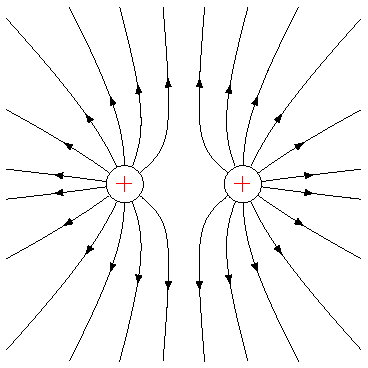
\includegraphics[width=5.5cm]{documents/figures/electric-field-lines-3b.pdf}
    \else
    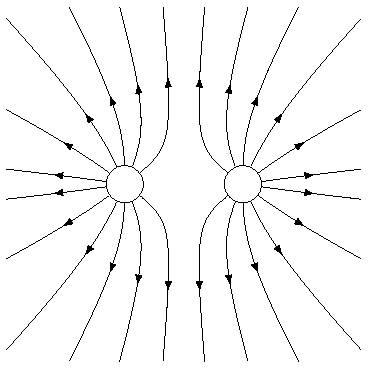
\includegraphics[width=5.5cm]{documents/figures/electric-field-lines-3a.pdf}
    \fi
    }
\end{minipage}%
\hspace{5mm}
\begin{minipage}{7cm}
    \centering
    \fbox{
    \ifprintanswers
    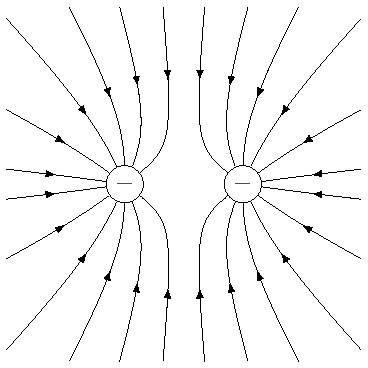
\includegraphics[width=5.5cm]{documents/figures/electric-field-lines-4b.pdf}
    \else
    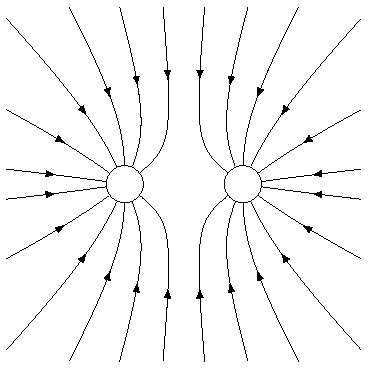
\includegraphics[width=5.5cm]{documents/figures/electric-field-lines-4a.pdf}
    \fi
    }
\end{minipage}
\end{center}

\begin{center}
\begin{minipage}{7cm}
    \centering
    \fbox{
    \ifprintanswers
    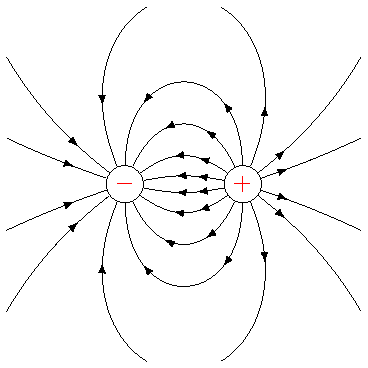
\includegraphics[width=5.5cm]{documents/figures/electric-field-lines-5b.pdf}
    \else
    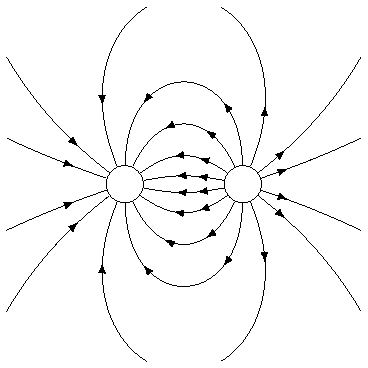
\includegraphics[width=5.5cm]{documents/figures/electric-field-lines-5a.pdf}
    \fi
    }
\end{minipage}%
\hspace{2.5mm}
\begin{minipage}{3.5cm}
    \fbox{
    \begin{tikzpicture}[x=1.5cm,y=1.5cm]
        \begin{scope}[decoration={
            markings,
            mark=at position 0.6 with {\arrow{>}}}
            ] 
        \foreach \x in {0,45,...,315}{
            \draw[postaction={decorate},rotate=\x] (0,0) -- (1,0);
        }
        \end{scope}
        \draw[fill=white] (0,0) circle (3mm) node {\ifprintanswers \textcolor{red}{\large $+$} \else \fi};
    \end{tikzpicture}
    }
\end{minipage}%
\hspace{2.5mm}
\begin{minipage}{3.5cm}
    \fbox{
    \begin{tikzpicture}[x=1.5cm,y=1.5cm]
        \begin{scope}[decoration={
            markings,
            mark=at position 0.6 with {\arrow{<}}}
            ] 
        \foreach \x in {0,45,...,315}{
            \draw[postaction={decorate},rotate=\x] (0,0) -- (1,0);
        }
        \end{scope}
        \draw[fill=white] (0,0) circle (3mm) node {\ifprintanswers \textcolor{red}{\large $-$} \else \fi};
    \end{tikzpicture}
    }
\end{minipage}
\end{center}

\end{questions}

\clearpage

\textbf{\Large Transfer of Charge}


\clearpage

\textbf{\Large Coulomb’s Law}

\subsection{Electric Force, Charges, and Distance}

\begin{questions}
% \question
% Google the \textit{PhET Simulation} called \texttt{Coulomb's law} (or \href{https://phet.colorado.edu/en/simulations/coulombs-law}{click here}). Press \texttt{Play}, and select the \texttt{Macro Scale} panel. This simulation helps you understand Coulomb's law. (a) How does the magnitude and direction of the force on $q_1$ by $q_2$ compare to that of the force on $q_2$ by $q_1$? (b) What changes in the simulation cause the magnitude of the forces to increase? (c) What changes cause the magnitude of the force to decrease? (d) What changes cause the direction of the forces to change?

\question
Object A has a positive charge of \SI{6.0e-6}{C}. Object B has a positive charge of \SI{3.0e-6}{C}. The two objects are 0.03 meters apart. Calculate the electric force between the two objects. 

\begin{solution}
\begin{equation*}
    F_e = \frac{k\left|q_1 q_2\right|}{r^2} = \frac{\left(\SI{9e9}{N\cdot m^2/C^2}\right)(\SI{6.0e-6}{C})(\SI{3.0e-6}{C})}{\left(\SI{0.03}{m}\right)^2} = \boxed{\SI{180}{N}}
\end{equation*}
\end{solution}

\question
Two positive charges of \SI{6.0e-6}{C} are separated by 0.50 meters. Calculate the electric force between the two objects. 

\begin{solution}
\begin{equation*}
    F_e = \frac{k\left|q_1 q_2\right|}{r^2} = \frac{\left(\SI{9e9}{N\cdot m^2/C^2}\right)\left(\SI{6.0e-6}{C}\right)^2}{\left(\SI{0.50}{m}\right)^2} = \boxed{\SI{1.296}{N}}
\end{equation*}
\end{solution}

\question
A negative charge of \SI{-6.0e-6}{C} exerts an attractive force of \SI{65}{N} on a second charge 0.05 meters away. What is the magnitude of the second charge?

\begin{solution}
Coulomb's law is

\begin{equation*}
    F_e = \frac{k\left|q_1q_2\right|}{r^2}
\end{equation*}

We know all variables except for $q_2$, which we can solve for algebraically as follows: Multiplying both sides by $r^2$ gives

\begin{equation*}
    F r^2 = k |q_1 q_2|
\end{equation*}

Dividing both sides by the produce $k q_1$ gives

\begin{equation*}
    |q_2| = \frac{F r^2}{k |q_1|} = \frac{(\SI{65}{N})(\SI{0.05}{m})^2}{(\SI{9e9}{N\cdot m^2/C^2})|(-\SI{6.0e-6}{C})|} = \boxed{\SI{3.0e-6}{C}}
\end{equation*}
\end{solution}

\question 
A force of \SI{-4.4e3}{N} exists between a positive charge of \SI{8.0e-4}{C} and a negative charge of \SI{-3.0e-4}{C}. What distance separates the charges?

\begin{solution}
Coulomb's law is

\begin{equation*}
    F = \frac{k q_1 q_2}{r^2}
\end{equation*}

Solving for distance leads to

\begin{equation*}
    r = \sqrt{\frac{kq_1q_2}{F}} = \sqrt{\frac{(\SI{9e9}{N\cdot m^2/C^2})(\SI{8.0e-4}{C})(\SI{-3.0e-4}{C})}{-\SI{4.4e3}{N}}} = \boxed{\SI{0.70}{m}} = \SI{70}{cm}
\end{equation*}
\end{solution}


\question \label{z4pMlx}
Two objects with charges \SI{7}{\micro C} and \SI{5}{\micro C} are separated by \SI{2}{cm}. (a) Is the electric force between them attractive or repulsive? (b) What is the magnitude of the electric force between the spheres?

\begin{solution}
(a) Repulsive. 

(b) \SI{786.6}{N}
\end{solution}


\question \label{TPIAio}
Two metallic spheres with charges \SI{-7}{\micro C} and \SI{5}{\micro C} are separated by \SI{2}{cm}. (a) Do the spheres attract each other, or do they repel? (b) What is the magnitude of the electric force between the spheres?

\begin{solution}
(a) Attract. 

(b) \SI{786.6}{N}
\end{solution}


\question \label{mJu5SD}
As shown below, two charges are placed near each other. (a) Are they attracted or repulsed? (b) What is the magnitude of the electric force between the charges?
\vspace{-1em}

\begin{center}
\begin{tikzpicture}
\begin{axis}[width=8cm,height=3.7cm,
clip=false,
xmin=-2.1,xmax=4,ymin=-0.6,ymax=1.2,
axis line style={draw=none},
ticks=none,    
]
\fill (0,0) circle (2pt);
\draw (0,0) circle (6mm) node[above=6mm] {\SI{8}{\micro C}};

\begin{scope}[xshift=3.01*1.07 cm]
    \fill (0,0) circle (2pt);
    \draw (0,0) circle (6mm) node[above=6mm] {\SI{9}{\micro C}};
\end{scope}

\draw[<->,dashed] (0,0.2) -- ++(axis direction cs: 3.01,0);
\node[above=6pt] at (3.01/2,0) {\SI{6}{cm}};
\end{axis}
\end{tikzpicture}
\end{center}

\begin{solution}
(a) Repulsed. (b) \SI{179.8}{N}
\end{solution}


\question \label{NqU30G}
(a) Are the charges below attracted or repulsed by each other? (b) Calculate the electrostatic force between them.
\vspace{-1em}

\begin{center}
\begin{tikzpicture}
\begin{axis}[width=8cm,height=3.7cm,
clip=false,
xmin=-2.1,xmax=4,ymin=-0.6,ymax=1.2,
axis line style={draw=none},
ticks=none,    
]
\fill (0,0) circle (2pt);
\draw (0,0) circle (6mm) node[above=6mm] {\SI{-3.2}{\micro C}};

\begin{scope}[xshift=3.01*1.07 cm]
    \fill (0,0) circle (2pt);
    \draw (0,0) circle (6mm) node[above=6mm] {\SI{-2.5}{\micro C}};
\end{scope}

\draw[<->,dashed] (0,0.2) -- ++(axis direction cs: 3.01,0);
\node[above=6pt] at (3.01/2,0) {\SI{1.4}{cm}};
\end{axis}
\end{tikzpicture}
\end{center}

\begin{solution}
\SI{366.9}{N}
\end{solution}


\question \label{S2QW5m}
When the two opposite charges shown below are placed near each other, the magnitude of the electrostatic force is \SI{44}{N}. What is the distance between the charges?

\begin{center}
\begin{tikzpicture}
\begin{axis}[width=8cm,height=3.7cm,
clip=false,
xmin=-0.5,xmax=6,ymin=-0.6,ymax=1.2,
axis line style={draw=none},
ticks=none,    
]
\fill (0,0) circle (3pt);
\draw (0,0) circle (6mm) node[above=6mm] {\SI{-680}{\micro C}};
\draw[->,thick] (0,0) -- ++(axis direction cs: 2,0) node[below] {$\SI{44}{N}$};

\begin{scope}[xshift=5.02*0.99 cm]
    \fill (0,0) circle (3pt);
    \draw (0,0) circle (6mm) node[above=6mm] {\SI{180}{\micro C}};
    \draw[->,thick] (0,0) -- ++(axis direction cs: -2,0); %node[below] {$F$};
\end{scope}

\draw[<->,dashed] (0,0.2) -- ++(axis direction cs: 5.02,0);
\node[above=6pt] at (5.02/2,0) {$r =\ ?$};
\end{axis}
\end{tikzpicture}
\end{center}

\begin{solution}
\SI{5.0}{m}
\end{solution}


\question \label{clmO0M}
A \SI{-48}{\micro C} charge and a \SI{55}{\micro C} one are separated by an unknown distance. If the electrostatic force between the charges is \SI{8.2}{N}, what is the distance between the charges?

\begin{solution}
\SI{1.7}{m}
\end{solution}

\question \label{TrRzFe}
Calculate the distance between the charges below if the force $F$ is \SI{7.52e-3}{N}.

\begin{center}
\begin{tikzpicture}
\begin{axis}[width=8cm,height=3.7cm,
clip=false,
xmin=-0.5,xmax=6,ymin=-0.6,ymax=1.2,
axis line style={draw=none},
ticks=none,    
]
\fill (0,0) circle (3pt);
\draw (0,0) circle (6mm) node[above=6mm] {\SI{-860}{\micro C}};
\draw[->,thick] (0,0) -- ++(axis direction cs: 2,0) node[below] {$F$};

\begin{scope}[xshift=5.02*0.99 cm]
    \fill (0,0) circle (3pt);
    \draw (0,0) circle (6mm) node[above=6mm] {\SI{420}{\micro C}};
    \draw[->,thick] (0,0) -- ++(axis direction cs: -2,0); %node[below] {$F$};
\end{scope}

\draw[<->,dashed] (0,0.2) -- ++(axis direction cs: 5.02,0);
\node[above=6pt] at (5.02/2,0) {$r =\ ?$};
\end{axis}
\end{tikzpicture}
\end{center}

\begin{solution}
\SI{657}{m}
\end{solution}


\question \label{bpbHHg}
When a 0.0066-coulomb charge is placed near a 0.0044-coulomb one, they experience a mutual repulsive force with a magnitude of 74 newtons. What is the distance between the charges?

\begin{solution}
\SI{59.4}{m}
\end{solution}



\question \label{DOuqpT}
Solve Exercise \ref{TrRzFe} analytically, which means using
only algebraic symbols and manipulation, and no numbers. Your result should be an equation solved for $r$ in terms of $F$, $k$, $q_1$, and $q_2$.

\begin{solution}
$r = \sqrt{\frac{k |q_1 q_2|}{F}}$
\end{solution}

\end{questions}


\clearpage

\subsection{How Changing Charge or Distance Affects the Electric Force}

\begin{questions}

\question
Two charged objects have a repulsive force of \SI{0.080}{N}. If the charge of one of the objects is doubled, then what is the new force?

\begin{solution}
The ratio of the new force to the old force is

\begin{equation*}
    \frac{F}{F_0} = \frac{(1)(1)(2)}{(1)^2} = 2
\end{equation*}

Therefore,

\begin{equation*}
    F = 2F_0 = \boxed{\SI{0.16}{N}}
\end{equation*}

\end{solution}



\question
Two charged objects have a repulsive force of \SI{0.080}{N}. If the charge of both of the objects is doubled, then what is the new force?

\begin{solution}
$\SI{0.32}{N}$
\end{solution}

\question
Two charged objects have a repulsive force of \SI{0.080}{N}. If the distance separating the objects is doubled, then what is the new force?

\begin{solution}
$\SI{0.020}{N}$
\end{solution}

\question
Two charged objects have a repulsive force of \SI{0.080}{N}. If the distance separating the objects is tripled, then what is the new force?

\begin{solution}
$\SI{0.0088}{N}$
\end{solution}


\question
Two charged objects have a attractive force of \SI{0.080}{N}. If the distance separating the objects is quadrupled, then what is the new force?

\begin{solution}
$\SI{0.005}{N}$
\end{solution}

\question
Two charged objects have a attractive force of \SI{0.080}{N}. If the distance separating the objects is halved, then what is the new force?

\begin{solution}
\begin{equation*}
    \frac{F}{F_0} = \frac{(1)(1)(1)}{\left(\frac{1}{2}\right)^2} = \frac{1}{\frac{1}{2}\cdot\frac{1}{2}} = \frac{1}{\frac{1}{4}} = 4
\end{equation*}

\begin{equation*}
    F = 4 F_0 = 4(\SI{0.08}{N}) = \boxed{\SI{0.32}{N}}
\end{equation*}
\end{solution}

\question
Two charged objects have a repulsive force of \SI{0.080}{N}. If the charge of one of the objects is doubled, and the distance separating the objects is doubled, then what is the new force?

\begin{solution}
$\SI{0.04}{N}$
\end{solution}


\question
Two charged objects have a repulsive force of \SI{0.080}{N}. If the charge of both of the objects is doubled, and the distance separating the objects is doubled, then what is the new force?

\begin{solution}
$\SI{0.08}{N}$
\end{solution}

\question
Two charged objects have a attractive force of \SI{0.080}{N}. If the charge of one of the objects is increased by a factor of four, and the distance separating the objects is doubled, then what is the new force?

\begin{solution}
$\SI{0.08}{N}$
\end{solution}

\question
Two charged objects have a attractive force of \SI{0.080}{N}. If the charge of one of the objects is tripled, and the distance separating the objects is tripled, then what is the new force?

\begin{solution}
$\SI{0.0267}{N}$
\end{solution}








\question
A balloon with a charge of \SI{4.0e-5}{C} is held a distance of \SI{0.10}{m} from a second balloon having the same charge. Calculate the magnitude of the repulsive force.

\begin{solution}
\begin{equation*}
    F = \frac{kq_1q_2}{r^2} = \SI{1440}{N}
\end{equation*}
\end{solution}

\question
Calculate the electrical force (in Newtons) exerted between a 22-gram with a charge of \SI{-2.6e-6}{\micro\coulomb} and a wool sweater with a charge of $+\SI{3.8}{\micro\coulomb}$. The separation distance is \SI{0.75}{m}.

\begin{solution}
\begin{equation*}
    F = \frac{k q_1 q_2}{r^2} = \SI{0.158}{N}
\end{equation*}
\end{solution}

\question
Suppose that two equally charged spheres attract each other with a force of \SI{-0.492}{N} (the negative sign indicating an attractive force) when placed a distance of \SI{29.1}{cm} from each other. Determine the charge of the spheres. 

\begin{solution}
Let $q$ be magnitude of the charge on each sphere. Then Coulomb's law gives

\begin{equation*}
    F = \frac{kq^2}{r^2}
\end{equation*}

Solving for $q$ leads to 

\begin{equation*}
    q = \sqrt{\frac{Fr^2}{k}} = \boxed{\SI{2.15e-6}{C}}
\end{equation*}
\end{solution}

\question
A $+\SI{5.0}{\micro\coulomb}$ charge and a $-\SI{6.0}{\micro\coulomb}$ charge experience an attractive force of $-\SI{0.72}{N}$ (the negative sign indicating an attractive force). Determine their separation distance.

\begin{solution}
Coulomb's law states

\begin{equation*}
    F = \frac{kq_1q_2}{r^2}
\end{equation*}

Solving for distance gives

\begin{equation*}
    r = \sqrt{\frac{kq_1q_2}{F}} = \boxed{\SI{0.61}{m}}
\end{equation*}
\end{solution}
\end{questions}

\clearpage



\textbf{\Large Simple Circuits}

\subsection{Electric Current}

\begin{questions}
\question
A lightbulb is connect with wires to a battery. The electrons flow out of the \fillin[negative ] terminal and into the \fillin[positive ] terminal.


\question
What is electric current?

\begin{randomizechoices}
    \correctchoice \glsdesc{electric current}
    \choice \glsdesc{resistance}
\end{randomizechoices}


\question
The SI unit of electric current is the \dots\ .


\question
How can you express 1 \textit{ampere} in terms of a \textit{coulomb} and a \textit{second}?


\question
To calculate electric current, according to some equation, you should compute \dots\ in units of \dots\ divided by \dots\ in units of \dots .


\question
To help you understand the flow of electrons in electric current, what is the analogy provided in the text? Draw a sketch of this analogy.


\question
Give an example of a machine or device that uses a large current.


\question
Give an example of a machine or device that uses a small current.


\question
It takes 3.5 nanoseconds for 14 nanocoulombs of charge to flow through a section of a wire. Calculate the magnitude of electric current flowing through the wire.


\question
A total charge of \qty{0.0035}{C} flows through a component of a car's engine in a time interval of \qty{0.2}{s}. What is the magnitude of the electric current through the component?

\end{questions}

\clearpage

\subsection{Components for a Simple Circuit}

For the following exercises, please access the \href{https://phet.colorado.edu/sims/html/circuit-construction-kit-dc/latest/circuit-construction-kit-dc_en.html}{PhET Simulation: Circuit Construction Kit}. Click the Intro tab, and check the box called Labels.

\begin{questions}


% \question
%     \href{https://photos.app.goo.gl/ntKqo9sznG9w7FiUA}{Click here} to view a photo of a real-world circuit. Then use \texttt{PhET} to simulation the circuit, which consists of two batteries, a switch, a lamp, and an ammeter, in series.
% 

\question
The following circuit diagram represents a circuit ``in series.'' Copy this sketch in your notebook. Then create the circuit in the PhET Simulation. Then copy it in your notebook, labeling it ``Parallel Circuit.''


\begin{center}
\begin{circuitikz}
\draw (0,0) to[bulb,l_={\SI{8}{\ohm}}]  (3,0) to[bulb,l_={\SI{12}{\ohm}}]  (3,2)
      (0,2) to[battery1,l_=\SI{36}{V}] (0,0)
      (0,2) to[cute closed switch] (3,2);
\end{circuitikz}
\end{center}

\question
Place an ammeter \textit{near} (not \textit{on}) the circuit. Then click-and-drag the crosshairs onto the wire to measure the current throughout all sections of wire.

The current in the circuit is \fillin[\SI{1.80}{A}].

\question
Does the current change throughout different portions of wire in the series circuit? \fillin[No][3cm]

\question
The total current in the circuit is the current flowing out of the positive terminal of the battery.

\begin{parts}
\part \label{abc123}
What is the total current? (\textit{Hint:} Use the ammeter.) \fillin[\SI{1.80}{A}][3cm]

\part Find the total (equivalent) resistance in the circuit. 

\begin{solutionorbox}[3cm]
For resistors in series, 

\begin{align*}
    R_{\mathrm{eq}} &= R_1 + R_2 \\[1ex]
    &= \SI{8}{\ohm} + \SI{12}{\ohm} \\[1ex]
    &= \boxed{\SI{20}{\ohm}}
\end{align*}
\end{solutionorbox}

\part Use Ohm's law to show that connecting the battery's voltage to the total resistance produces the total current measured in part~(\ref{abc123}). 

\begin{solutionorbox}[3cm]
By Ohm's law

\begin{align*}
    I &= \frac{V}{R_\mathrm{eq}} \\[1ex]
    &= \frac{\SI{36}{V}}{\SI{20}{\ohm}} \\[1ex]
    &= \boxed{\SI{1.80}{A}}
\end{align*}

This is the same current measured by the ammeter.
\end{solutionorbox}

\end{parts}

\question
The following circuit is constructed ``in parallel'' because electrons can branch out to either light bulb at the junction. Open a new internet tab, and recreate this parallel circuit in the PhET Simulation. 


\begin{center}
\begin{tikzpicture}[x=1.5cm,y=1.8cm]
    \draw (0,1) to[battery1,l_={\SI{36}{V}}] (0,0) -- (4,0) to[bulb,l_={\SI{12}{\ohm}}] (4,1) ;
    \draw (2,1) to[bulb={\SI{8}{\ohm}}] (2,0);
    \draw (0,1) to[cute closed switch] (2,1) to[cute closed switch] (4,1);
    \draw[thick,<-,yshift=2pt] (2,1) -- ++(0,0.4) node[above] {Junction};
\end{tikzpicture}
\end{center}
 
\question
Place an ammeter near the circuit. Again, use the crosshairs to measure the current throughout all sections of wire. You may open and close the switches as needed in your investigation.

In your notebook sketch, label the current in amperes (A) through various portions of wire in the circuit.


\question
Does the current change throughout the parallel circuit? \fillin[Yes].

\question
The total current in the circuit is the current coming out of the positive terminal of the battery. This total current is distributed across each ``branch'' of the circuit.

\begin{parts}
\part Use the ammeter to measure the total current? \fillin[\SI{7.50}{A}][3cm].
\part Again, use the ammeter to measure the current through the \SI{8}{\ohm} resistor. \fillin[\SI{4.50}{A}][3cm]
\part Measure the current through the \SI{12}{\ohm} resistor. \fillin[\SI{3.00}{A}][3cm]

\part Find a mathematical relationship between the currents through the resistor and the total current in the circuit.

\begin{solutionorbox}
The total current is \SI{7.5}{A}, and the currents through each of the two resistors are \SI{4.5}{A} and \SI{3.0}{A}. Thus the relationship is

\begin{equation*}
    \SI{4.5}{A} + \SI{3.0}{A} = \SI{7.5}{A}
\end{equation*}

That is, the sum of the currents across each resistor equals the total current in the circuit.
\end{solutionorbox}
\end{parts}



\question
\begin{parts}
\part Find the total (equivalent) resistance in the circuit. 

\begin{solutionorbox}[3cm]
For resistors in series, 


\end{solutionorbox}


\part Use Ohm's law to show that connecting the battery's voltage to the total resistance produces the total current measured in part~(\ref{abc123}).

\begin{solutionorbox}[3cm]

\end{solutionorbox}

\end{parts}
\end{questions}

\clearpage

\subsection{Circuits in Series}

\begin{questions}
\question
Go to PhET Simulation: Circuit Construction Kit and build the circuit shown below. Points a through h are labeled for referencing current or voltages at those points. For example, $I_\mathrm{b}$ is the current through Point b, and $V_\mathrm{de}$ is the voltage (or potential difference) across Points d and e.

Use the ammeter and voltmeters in the simulation to measure currents and voltages at or across the specified points, and record your values below:

\begin{center}
% \fbox{
\begin{minipage}{5.5cm}
\centering
\begin{tikzpicture}[x=3cm,y=2.5cm]
    \draw (0,1) to[battery1,l_={\SI{5}{V}}] (0,0) to[R,l_={$R_2 = \SI{3}{\ohm}$}] (1,0) to[R={$R_1$},n=R1,-o]  (1,1)  -- (0,1);
    \draw (R1.s) node[right]{\SI{2}{\ohm}};
    \fill (0,0.75) circle (2pt) node[left=1pt] {a};
    \fill (0.25,1) circle (2pt) node[above=1pt] {b};
    \fill (0.75,1) circle (2pt) node[above=1pt] {c};
    \fill (1,0.75) circle (2pt) node[right=1pt] {d};
    \fill (1,0.25) circle (2pt) node[right=1pt] {e};
    \fill (0.75,0) circle (2pt) node[above=1pt] {f};
    \fill (0.25,0) circle (2pt) node[above=1pt] {g};
    \fill (0,0.25) circle (2pt) node[left=1pt] {h};
\end{tikzpicture}
\end{minipage}
%}
\fbox{
\begin{minipage}{4.0cm}
\centering
\begin{align*}
    I_\mathrm{b} &= {\ifprintanswers \color{red} \else \color{white} \fi {\SI{1.00}{A}} }  \\[1ex]
    I_\mathrm{e} &= {\ifprintanswers \color{red} \else \color{white} \fi {\SI{1.00}{A}} }  \\[1ex]
    I_\mathrm{g} &= {\ifprintanswers \color{red} \else \color{white} \fi {\SI{1.00}{A}} }  
\end{align*}
\end{minipage}}
\fbox{
\begin{minipage}{4.0cm}
\centering
\begin{align*}
    V_\mathrm{de} &= {\ifprintanswers \color{red} \else \color{white} \fi {\SI{-2.00}{V}} }  \\[1ex]
    V_\mathrm{fg} &= {\ifprintanswers \color{red} \else \color{white} \fi {\SI{-3.00}{V}} }  \\[1ex]
    V_\mathrm{ha} &= {\ifprintanswers \color{red} \else \color{white} \fi {\SI{5.00}{V}} }  \\[1ex]
    V_\mathrm{gc} &= {\ifprintanswers \color{red} \else \color{white} \fi {\SI{5.00}{V}} }  
\end{align*}
\end{minipage}}
\end{center}

\begin{parts}
    \part What is the voltage drop across resistor $R_1$? \fillin[\SI{-2.00}{V}]
    \part What is the voltage drop across resistor $R_2$? \fillin[\SI{-3.00}{V}]
    \part Measure the potential difference (or voltage) across the battery. \fillin[\SI{5.00}{V}]
    \part Find the total resistance in circuit. \fillin[\SI{5.00}{\ohm}]
    \part What is the total current? \fillin[\SI{1.00}{A}]
\end{parts}


\question
\phantom{.}

\begin{center}
% \fbox{
\begin{minipage}{9.5cm}
\centering
\begin{tikzpicture}[x=2.5cm,y=2cm]
    \draw (0,1) to[battery1,l_={\SI{5}{V}}] (0,0);
    \draw (0,1) to[R={$R_1$},n=R1] (1,1) to[R={$R_2$},n=R2] (2,1) to[R={$R_3$},n=R3] (3,1) -- (3,0) -- (0,0);
    \draw (R1.s) node[below] {\SI{2}{\ohm}};
    \draw (R2.s) node[below] {\SI{2}{\ohm}};
    \draw (R3.s) node[below] {\SI{1}{\ohm}};
    \fill (0,0.75) circle (2pt) node[left=1pt] {a};
    \fill (0.2,1) circle (2pt) node[above=1pt] {b};
    \fill (0.8,1) circle (2pt) node[above=1pt] {c};
    \fill (1.2,1) circle (2pt) node[above=1pt] {d};
    \fill (1.8,1) circle (2pt) node[above=1pt] {e};
    \fill (2.2,1) circle (2pt) node[above=1pt] {f};
    \fill (2.8,1) circle (2pt) node[above=1pt] {g};
    \fill (3,0.8) circle (2pt) node[right=1pt] {h};
    \fill (3,0.2) circle (2pt) node[right=1pt] {i};
    \fill (1.5,0) circle (2pt) node[above=1pt] {j};
    \fill (0,0.2) circle (2pt) node[left=1pt] {k};
\end{tikzpicture}
\end{minipage}
% }
\fbox{
\begin{minipage}{5cm}
\centering
\begin{align*}
    I_\mathrm{b} &= {\ifprintanswers \color{red} \else \color{white} \fi {\SI{1.00}{A}} }  \\[1ex]
    I_\mathrm{c} &= {\ifprintanswers \color{red} \else \color{white} \fi {\SI{1.00}{A}} }  \\[1ex]
    I_\mathrm{f} &= {\ifprintanswers \color{red} \else \color{white} \fi {\SI{1.00}{A}} }  \\[1ex]
    I_\mathrm{j} &= {\ifprintanswers \color{red} \else \color{white} \fi {\SI{1.00}{A}} }  \\[1ex]
    V_\mathrm{ka} &= {\ifprintanswers \color{red} \else \color{white} \fi {\SI{5.00}{V}} }  \\[1ex]
    V_\mathrm{hi} &= {\ifprintanswers \color{red} \else \color{white} \fi {\SI{0.00}{V}} }  
\end{align*}
\end{minipage}
}
\end{center}

\begin{parts}
    \part Calculate the total resistance in the circuit. \fillin[\SI{6}{\ohm}]
    \part What is the total current in the circuit? \fillin[\SI{1.00}{A}]
    \part Measure the voltage drop across resistor $R_1$. \fillin[\SI{-2.00}{V}]
    \part What is the voltage drop across resistor $R_2$? \fillin[\SI{-2.00}{V}]
    \part What is the potential difference across resistor $R_3$? \fillin[\SI{-1.00}{V}]
\end{parts}

\question
\phantom{.}

\begin{center}
\begin{tikzpicture}[x=2.5cm,y=2.5cm]
    \draw (0,1) to[battery1,l_={\SI{3}{V}}] (0,0);
    \draw (0,1) to[R={$R_1$},n=R1] (1,1) to[R={$R_2$},n=R2] (1,0) -- (0,0);
    \fill (0,0.75) circle (2pt) node[left=1pt] {a};
    \fill (0.25,1) circle (2pt) node[above=1pt] {b};
    \fill (0.75,1) circle (2pt) node[above=1pt] {c};
    \fill (1,0.75) circle (2pt) node[right=1pt] {d};
    \fill (1,0.25) circle (2pt) node[right=1pt] {e};
    \fill (0.75,0) circle (2pt) node[below=1pt] {f};
    \fill (0,0.25) circle (2pt) node[left=1pt] {g};
    \draw (R1.s) node[below] {\SI{5}{\ohm}};
    \draw (R2.s) node[left] {\SI{1}{\ohm}};
\end{tikzpicture}
\end{center}

\question
\phantom{.}

\begin{center}
\begin{tikzpicture}[x=2.5cm,y=2cm]
    \draw (0,1) to[battery1,l_={\SI{6}{V}}] (0,0);
    \draw (0,1) to[R,l={$R_1 = \SI{5}{\ohm}$}] (1,1) to[R,l={$R_2 = \SI{1}{\ohm}$}] (1,0) to[R={$R_3 = \SI{2}{\ohm}$}] (0,0);
\end{tikzpicture}
\end{center}

\end{questions}


\clearpage

\subsection{Circuits in Parallel}

\begin{questions}
\question
\phantom{.}

\begin{center}
\fbox{
\begin{minipage}{6.5cm}
    \begin{tikzpicture}[x=2.5cm,y=2cm]
        \draw (0,1) to[battery1,l={\SI{10}{V}}] (0,0);
        \draw (0,0) -- (2,0) to[R={$R_2$},n=R2] (2,1) -- (0,1);
        \draw (1,0) to[R={$R_1$},n=R1] (1,1);
        \draw (R1.s) node[right] {\SI{2}{\ohm}};
        \draw (R2.s) node[right] {\SI{4}{\ohm}};
        \fill (0,0.8) circle (2pt) node[left=1pt] {a};
        \fill (0.5,1) circle (2pt) node[above=1pt] {b};
        \fill (2,0.8) circle (2pt) node[right=1pt] {c};
        \fill (2,0.2) circle (2pt) node[right=1pt] {d};
        \fill (0.5,0) circle (2pt) node[below=1pt] {e};
        \fill (1,0.8) circle (2pt) node[right=1pt] {f};
        \fill (1,0.2) circle (2pt) node[right=1pt] {g};
        \fill (0,0.2) circle (2pt) node[left=1pt] {h};
    \end{tikzpicture}
\end{minipage}
}
\fbox{
\begin{minipage}{4cm}
    \begin{align*}
        I_\mathrm{g} &= {\ifprintanswers \color{red} \else \color{white} \fi {\SI{5.00}{A}} } \\[1ex]
        I_\mathrm{d} &= {\ifprintanswers \color{red} \else \color{white} \fi {\SI{2.50}{A}} } \\[1ex]
        I_\mathrm{b} &= {\ifprintanswers \color{red} \else \color{white} \fi {\SI{7.50}{A}} } \\[1ex]
        I_\mathrm{e} &= {\ifprintanswers \color{red} \else \color{white} \fi {\SI{7.50}{A}} } \\[1ex]
        V_\mathrm{ha} &= {\ifprintanswers \color{red} \else \color{white} \fi {\SI{10.00}{A}} } 
    \end{align*}
\end{minipage}
}
\end{center}

\begin{parts}
\part What is the equivalent resistance of the circuit? \fillin[\SI{1.33}{\ohm}]
\part What is the current through resistor $R_1$? \fillin[\SI{5.00}{A}]
\part Measure the current through resistor $R_2$. \fillin[\SI{2.50}{A}]
\part Find the total current in the circuit. \fillin[\SI{7.50}{A}]
\part What is the voltage drop across $R_1$? \fillin[\SI{10}{V}]
\part What is the voltage drop across $R_2$? \fillin[\SI{10}{V}]
\end{parts}

\question
\phantom{.}

\begin{center}
\begin{tikzpicture}[x=2.5cm,y=2cm]
    \draw (0,1) to[battery1,l={\SI{12}{V}}] (0,0);
    \draw (0,0) -- (3,0) to[R={$R_3$},n=R3] (3,1) -- (0,1);
    \draw (1,0) to[R={$R_1$},n=R1] (1,1);
    \draw (2,0) to[R={$R_2$},n=R2] (2,1);
    \draw (R1.s) node[right] {\SI{2}{\ohm}};
    \draw (R2.s) node[right] {\SI{4}{\ohm}};
    \draw (R3.s) node[right] {\SI{3}{\ohm}};
    \fill (0,0.8) circle (2pt) node[left=1pt] {a};
    \fill (0.5,1) circle (2pt) node[above=1pt] {b};
    \fill (3,0.8) circle (2pt) node[right=1pt] {c};
    \fill (3,0.2) circle (2pt) node[right=1pt] {d};
    \fill (1.5,0) circle (2pt) node[below=1pt] {e};
    \fill (0.5,0) circle (2pt) node[below=1pt] {f};
    \fill (0,0.2) circle (2pt) node[left=1pt] {g};
    \fill (1,0.8) circle (2pt) node[right=1pt] {h};
    \fill (1,0.2) circle (2pt) node[right=1pt] {i};
    \fill (2,0.8) circle (2pt) node[right=1pt] {j};
    \fill (2,0.2) circle (2pt) node[right=1pt] {k};
\end{tikzpicture}
\end{center}

\question
\phantom{.}

\begin{center}
\begin{tikzpicture}[x=2.5cm,y=2cm]
    \draw (0,1) to[battery1,l={\SI{8}{V}}] (0,0);
    \draw (0,0) -- (2,0) to[R={$R_2$},n=R2] (2,1) -- (0,1);
    \draw (1,0) to[R={$R_1$},n=R1] (1,1);
    \draw (R1.s) node[right] {\SI{10}{\ohm}};
    \draw (R2.s) node[right] {\SI{40}{\ohm}};
    \fill (0,0.8) circle (2pt) node[left=1pt] {a};
    \fill (0.5,1) circle (2pt) node[above=1pt] {b};
    \fill (2,0.8) circle (2pt) node[right=1pt] {c};
    \fill (2,0.2) circle (2pt) node[right=1pt] {d};
    \fill (0.5,0) circle (2pt) node[below=1pt] {e};
    \fill (1,0.8) circle (2pt) node[right=1pt] {f};
    \fill (1,0.2) circle (2pt) node[right=1pt] {g};
\end{tikzpicture}
\end{center}

\question
\phantom{.}

\begin{center}
\begin{tikzpicture}[x=2.5cm,y=2cm]
    \draw (0,1) to[battery1,l={\SI{5}{V}}] (0,0);
    \draw (0,0) -- (3,0) to[R={$R_3$},n=R3] (3,1) -- (0,1);
    \draw (1,0) to[R={$R_1$},n=R1] (1,1);
    \draw (2,0) to[R={$R_2$},n=R2] (2,1);
    \draw (R1.s) node[right] {\SI{10}{\ohm}};
    \draw (R2.s) node[right] {\SI{10}{\ohm}};
    \draw (R3.s) node[right] {\SI{10}{\ohm}};
    \fill (0,0.8) circle (2pt) node[left=1pt] {a};
    \fill (0.5,1) circle (2pt) node[above=1pt] {b};
    \fill (3,0.8) circle (2pt) node[right=1pt] {c};
    \fill (3,0.2) circle (2pt) node[right=1pt] {d};
    \fill (1.5,0) circle (2pt) node[below=1pt] {e};
    \fill (0.5,0) circle (2pt) node[below=1pt] {f};
    \fill (0,0.2) circle (2pt) node[left=1pt] {g};
    \fill (1,0.8) circle (2pt) node[right=1pt] {h};
    \fill (1,0.2) circle (2pt) node[right=1pt] {i};
    \fill (2,0.8) circle (2pt) node[right=1pt] {j};
    \fill (2,0.2) circle (2pt) node[right=1pt] {k};
\end{tikzpicture}
\end{center}

\end{questions}

\clearpage


\subsection{Resistors in Series and Parallel}

\textbf{Series Circuits}

\begin{questions}
\question 
In the circuit shown below, a voltage of \SI{6}{V} pushes charge through a single resistor of \SI{2}{\ohm}. According to Ohm's law, the current in the resistor (and therefore in the whole circuit) is \fillin[\SI{3}{A}].

\begin{center}
\begin{tikzpicture}[x=2cm,y=1.5cm]
    \draw (0,0) to[battery1,l_={\SI{6}{V}}] (1,0) -- (1,1) to[R,l_={\SI{2}{\ohm}}] (0,1) -- (0,0);
\end{tikzpicture}
\end{center}

\question
If a second identical resistor is added, as shown below, the \SI{6}{V} battery must push charge through a total resistance of \fillin[\SI{6}{\ohm}].
The current in the circuit is then \fillin[\SI{1}{A}].

\begin{center}
\begin{tikzpicture}[x=2cm,y=1.5cm]
    \draw (0,0) to[battery1,l_={\SI{6}{V}}] (1,0) to[R,l_={\SI{3}{\ohm}}] (1,1) to[R,l_={\SI{3}{\ohm}}] (0,1) -- (0,0);
\end{tikzpicture}
\end{center}


\question
The equivalent resistance of three \SI{4}{\ohm} resistors in series is \fillin[\SI{12}{\ohm}].

\question
Does current flow \textit{through} a resistor, or \textit{across} a resistor? \fillin[through]

Is voltage established \textit{through} a resistor, or \textit{across} a resistor? \fillin[across]


\question
Does current in the lamps occur simultaneously, or does charge flow first through one lamp, then the other, and finally the last in turn?

\fillin[Simultaneously\hfill][0.9\textwidth]



\question 
Circuits A and B below are identical with all bulbs rated at equal wattage (therefore equal resistance). The only difference between the circuits is that Bulb 5 has a short circuit, as shown.

\begin{center}
\begin{tikzpicture}[x=2cm,y=1.5cm]
    \draw (0,0) to[battery1,l_={\SI{4.5}{V}}] (3,0); 
    \draw (0,0) -- (0,1) to[bulb,l_=1] (1,1) to[bulb,l_=2] (2,1) to[bulb,l_=3] (3,1) -- (3,0);
    \node[above=2pt] at (current bounding box.north) {Circuit A};
\end{tikzpicture}
\hspace{5mm}
\begin{tikzpicture}[x=2cm,y=1.5cm]
    \draw (0,0) to[battery1,l_={\SI{4.5}{V}}] (3,0); 
    \draw (0,0) -- (0,1) to[bulb,l_=4] (1,1) to[bulb,l_=5] (2,1) to[bulb,l_=6] (3,1) -- (3,0);
    \draw[rounded corners=3mm] (1,1) -- (1.25,0.6) -- (1.5,0.4) -- (1.75,0.6) -- (2,1);
    \fill (1,1) circle (1pt);
    \fill (2,1) circle (1pt);
    \node[above=2pt] at (current bounding box.north) {Circuit B};
\end{tikzpicture}
\end{center}

\begin{parts}
\part In which circuit is the current greater? \fillin[B]
\part In which circuit are all three bulbs equally bright? \fillin[A]
\part What bulbs are the brightest? \fillin[4 and 6]
\part What bulb is the dimmest? \fillin[5]
\part What bulbs have the largest voltage drops across them? \fillin[4 and 6]
\part What circuit dissipates more power? \fillin[B]
\part What circuit produces more light? \fillin[B]
\end{parts}


\uplevel{\textbf{Parallel Circuits}}

\question
In the circuit shown below, there is a voltage drop of \SI{6}{V} across each \SI{2}{\ohm} resistor. Points a through j are labeled for reference.

\begin{center}
\begin{tikzpicture}[x=2cm,y=2.5cm]
    \draw (0,1) to[battery1,l_={\SI{6}{V}}] (0,0);
    \draw (0,1) -- (2,1) to[R={\SI{2}{\ohm}}] (2,0) -- (0,0);
    \draw (1,1) to[R={\SI{2}{\ohm}}] (1,0);
    \fill (0,0.8) circle (1.5pt) node[left] {a};
    \fill (0.5,1) circle (1.5pt) node[above] {b};
    \fill (1.5,1) circle (1.5pt) node[above] {c};
    \fill (2,0.8) circle (1.5pt) node[right] {d};
    \fill (2,0.2) circle (1.5pt) node[right] {e};
    \fill (1.5,0) circle (1.5pt) node[below] {f};
    \fill (0.5,0) circle (1.5pt) node[below] {g};
    \fill (0,0.2) circle (1.5pt) node[left] {h};
    \fill (1,0.8) circle (1.5pt) node[right] {i};
    \fill (1,0.2) circle (1.5pt) node[right] {j};
\end{tikzpicture}
\end{center}

\begin{parts}
\part By Ohm's law, the current in each resistor is \fillin[\SI{3}{A}].
\part The current through the battery, which is the sum of the currents in the resistors, is \fillin[\SI{6}{A}].
\part Record the current through each of the points labeled in the figure.

\begin{gather*}
    I_\mathrm{a} = {\ifprintanswers \color{red} \else \color{white} \fi \SI{6}{A}} \qquad
    I_\mathrm{b} = {\ifprintanswers \color{red} \else \color{white} \fi \SI{6}{A}} \qquad
    I_\mathrm{c} = {\ifprintanswers \color{red} \else \color{white} \fi \SI{3}{A}} \qquad
    I_\mathrm{d} = {\ifprintanswers \color{red} \else \color{white} \fi \SI{3}{A}} \qquad
    I_\mathrm{e} = {\ifprintanswers \color{red} \else \color{white} \fi \SI{3}{A}} \\[1ex]
    I_\mathrm{f} = {\ifprintanswers \color{red} \else \color{white} \fi \SI{3}{A}} \qquad
    I_\mathrm{g} = {\ifprintanswers \color{red} \else \color{white} \fi \SI{6}{A}} \qquad
    I_\mathrm{h} = {\ifprintanswers \color{red} \else \color{white} \fi \SI{6}{A}} \qquad
    I_\mathrm{i} = {\ifprintanswers \color{red} \else \color{white} \fi \SI{3}{A}} \qquad
    I_\mathrm{j} = {\ifprintanswers \color{red} \else \color{white} \fi \SI{3}{A}} 
\end{gather*}
\end{parts}

\question
Which circuit below is \textit{not} equivalent to the circuit from the previous question?

\begin{center}
\begin{tikzpicture}[x=1.3cm,y=3cm]
    \draw (0,1) to[battery1] (0,0) -- (1.5,0);
    \draw (0,1) -- (1.5,1) -- (2,0.75) to[R] (2,0.25) -- (1.5,0);
    \draw (1.5,1) -- (1,0.75) to[R] (1,0.25) -- (1.5,0);
    \node[above=2pt] at (current bounding box.north) {Circuit W};
\end{tikzpicture}
\hspace{2em}
\begin{tikzpicture}[x=1.3cm,y=3cm]
    \draw (0,1) to[battery1] (0,0);
    \draw (0,1) -- (2,1) -- (2,0) to[R] (1,0) -- (0,0);
    \draw (1,1) to[R] (1,0);
    \node[above=2pt] at (current bounding box.north) {Circuit X};
\end{tikzpicture}
\hspace{2em}
\begin{tikzpicture}[x=1.3cm,y=3cm]
    \draw (0,1) to[battery1] (0,0) -- (1.5,0) -- (1.5,0.25);
    \draw (0,1) -- (1.5,1) -- (1.5,0.75) -- (1,0.75) to[R] (1,0.25) -- (2,0.25) to[R] (2,0.75) -- (1.5,0.75);
    \node[above=2pt] at (current bounding box.north) {Circuit Y};
\end{tikzpicture}
\hspace{2em}
\begin{tikzpicture}[x=1.3cm,y=3cm]
    \draw (0,1) to[battery1] (0,0);
    \draw (0,1) -- (2,1) -- (2,0) to[R] (1,0) to[R] (0,0);
    \draw (1,1) -- (1,0);
    \node[above=2pt] at (current bounding box.north) {Circuit Z};
\end{tikzpicture}
\end{center}

\question 
Consider the parallel circuit below.

\begin{center}
\begin{tikzpicture}[x=2cm,y=2cm]
    \draw (0,1) to[battery1,l_={\SI{6}{V}}] (0,0);
    \draw (0,1) -- (2,1) to[R={\SI{2}{\ohm}}] (2,0) -- (0,0);
    \draw (1,1) to[R={\SI{1}{\ohm}}] (1,0);
    \draw (2,1) -- (3,1) to[R={\SI{2}{\ohm}}] (3,0) -- (2,0);
\end{tikzpicture}
\end{center}

\begin{parts}
\part The voltage drop across each resistor is \fillin[\SI{6}{V}].
\part Now consider the currents in each branch.

\begin{itemize}[topsep=0pt]
    \item The current through the \SI{2}{\ohm} resistor is \fillin[\SI{3}{A}].
    \item The current through the \SI{2}{\ohm} resistor is \fillin[\SI{3}{A}].
    \item The current through the \SI{1}{\ohm} resistor is \fillin[\SI{6}{A}].
\end{itemize}

\part The current through the battery, which equals the sum of the currents in each branch, is \fillin[\SI{12}{A}].

\part The equivalent resistance of the circuit equals \fillin[\SI{0.5}{\ohm}].

\end{parts}
\end{questions}

\clearpage

\subsection{The Circuit Lab}

\begin{questions}
\question \label{Q1}
Make a circuit with a battery, light bulb, and switch. Close the switch to make the light turn on, ensuring the circuit is connected correctly. 

\question
Disconnect the clips from the switch to use the free ends as probes and test the following items for conductivity. Write a C if the item is a conductor, or an I for if it's an insulator.

\begin{center}
    Paper \fillin[I][2em] \hspace{2em}
    Lock nut \fillin[C][2em] \hspace{2em}
    Penny \fillin[C][2em] \hspace{2em}
    Paperclip \fillin[C][2em] \hspace{2em}
    Glass \fillin[I][2em] \hspace{2em} \\[1ex]
    Plastic \fillin[I][2em] \hspace{2em}
    Cloth \fillin[I][2em] \hspace{2em}
    Wood \fillin[I][2em] \hspace{2em}
    Rubber \fillin[I][2em] \hspace{2em}
\end{center}


\question
Connect clips wires to both sides of the battery. Unscrew and remove a light bulb from the holder. Use the free ends of the clips as probes and connect them the different points on the battery shown below.

\begin{EnvUplevel}
\vspace{-1em}
\begin{center}
\begin{tikzpicture}
    \node at (0,0) {\resizebox{1cm}{!}{\faLightbulbO}}  node[above left=7mm] {A};
    \draw[shift={(-0.5,-0.5)},<-,very thick] (0,0) -- (-0.8,0) node[left] {$-$};
    \draw[shift={(0,-0.9)},<-,very thick] (0,0) -- (0,-0.8) node[below] {$+$};
    \draw[shift={(+0.5,-0.5)},<-,white,very thick] (0,0) -- (+0.8,0) node[right] {$-$};
    \draw[shift={(0,+0.9)},<-,white,very thick] (0,0) -- (0,0.4) -- (0.6,0.4) node[right] {$+$};
\end{tikzpicture}
\begin{tikzpicture}
    \node at (0,0) {\resizebox{1cm}{!}{\faLightbulbO}}  node[above left=7mm] {B};
    \draw[shift={(-0.5,-0.5)},<-,very thick] (0,0) -- (-0.8,0) node[left] {$-$};
    \draw[shift={(0,-0.9)},<-,very thick,white] (0,0) -- (0,-0.8) node[below] {$+$};
    \draw[shift={(+0.5,-0.5)},<-,very thick] (0,0) -- (+0.8,0) node[right] {$+$};
    \draw[shift={(0,+0.9)},<-,very thick,white] (0,0) -- (0,0.4) -- (0.6,0.4) node[right] {$+$};
\end{tikzpicture}
\begin{tikzpicture}
    \node at (0,0) {\resizebox{1cm}{!}{\faLightbulbO}}  node[above left=7mm] {C};
    \draw[shift={(-0.5,-0.5)},<-,very thick,white] (0,0) -- (-0.8,0) node[left] {$-$};
    \draw[shift={(0,-0.9)},<-,very thick] (0,0) -- (0,-0.8) node[below] {$-$};
    \draw[shift={(+0.5,-0.5)},<-,very thick] (0,0) -- (+0.8,0) node[right] {$+$};
    \draw[shift={(0,+0.9)},<-,very thick,white] (0,0) -- (0,0.4) -- (0.6,0.4) node[right] {$+$};
\end{tikzpicture}
\begin{tikzpicture}
    \node at (0,0) {\resizebox{1cm}{!}{\faLightbulbO}}  node[above left=7mm] {D};
    \draw[shift={(-0.5,-0.5)},<-,very thick,white] (0,0) -- (-0.8,0) node[left] {$-$};
    \draw[shift={(0,-0.9)},<-,very thick] (0,0) -- (0,-0.8) node[below] {$-$};
    \draw[shift={(+0.5,-0.5)},<-,very thick,white] (0,0) -- (+0.8,0) node[right] {$-$};
    \draw[shift={(0,+0.9)},<-,very thick] (0,0) -- (0,0.4) -- (0.6,0.4) node[right] {$+$};
\end{tikzpicture}
\end{center}
\end{EnvUplevel}

Which diagram above indicates the two parts of a light bulb that must be touched to complete the circuit? \fillin[B][2cm]

\question
Re-create the closed circuit from Question \ref{Q1} (battery, bulb, and switch in series). Draw the circuit diagram below.

\begin{center}
\bgroup
\ifprintanswers
\color{red}
\else
\color{white}
\fi

\begin{tikzpicture}[x=2cm,y=1.5cm]
    \draw (0,1) to[battery1] (0,0); 
    \draw (0,1) to[bulb] (1,1) -- (1,0) to[cute closed switch] (0,0);
\end{tikzpicture}
\egroup
\end{center}

What happens if you reverse the battery (by reversing the battery holder)?

\fillwithlines{8mm}

\question
Create the four circuits with the listed components, and draw the diagrams in the spaces below.

\begin{EnvUplevel}
\fbox{
\begin{minipage}{0.47\textwidth}
\textbf{Circuit 1:} battery, light bulb, switch.
\begin{center}
\bgroup
\ifprintanswers
\color{red}
\else
\color{white}
\fi

\begin{tikzpicture}[x=2.5cm,y=1.5cm]
    \draw (0,1) to[battery1] (0,0); 
    \draw (0,1) to[bulb] (1,1) -- (1,0) to[cute closed switch] (0,0);
\end{tikzpicture}
\egroup
\end{center}

What happens if you unscrew the lightbulb?

\vspace{3cm}
% \fillin[The bulb turns off, and the circuit is open.][7.5cm]

\end{minipage}
}%
\fbox{
\begin{minipage}{0.47\textwidth}
\textbf{Circuit 2:} battery, 2 light bulbs, switch.
\begin{center}
\bgroup
\ifprintanswers
\color{red}
\else
\color{white}
\fi

\begin{tikzpicture}[x=2.5cm,y=1.5cm]
    \draw (0,1) to[battery1] (0,0.5) to[battery1] (0,0); 
    \draw (0,1) to[bulb] (1,1) -- (1,0) to[cute closed switch] (0,0);
\end{tikzpicture}
\egroup
\end{center}

How does this light's brightness compare to\\Circuit1 ? Explain.

\vspace{2.5cm}

% \fillin[Voltage and current has increased.][7.5cm]
\end{minipage}
}
\end{EnvUplevel}

\clearpage

\begin{EnvUplevel}
\fbox{
\begin{minipage}{0.47\textwidth}
\textbf{Circuit 3:} 2 batteries, 1 light bulb, 1 switch
\begin{center}
\bgroup
\ifprintanswers
\color{red}
\else
\color{white}
\fi

\begin{tikzpicture}[x=2.5cm,y=1.5cm]
    \draw (0,1) to[battery1] (0,0); 
    \draw (0,1) to[bulb] (1,1) -- (1,0) to[cute closed switch] (0,0);
\end{tikzpicture}
\egroup
\end{center}

How does this light's brightness compare to\\Circuit 1? Explain.

\vspace{2cm}
% \fillin[The bulb turns off, and the circuit is open.][7.5cm]

\end{minipage}
}%
\fbox{
\begin{minipage}{0.47\textwidth}
\textbf{Circuit 4:} 2 batteries, 2 light bulbs, 1 switch
\begin{center}
\bgroup
\ifprintanswers
\color{red}
\else
\color{white}
\fi

\begin{tikzpicture}[x=2.5cm,y=1.5cm]
    \draw (0,1) to[battery1] (0,0.5) to[battery1] (0,0); 
    \draw (0,1) to[bulb] (1,1) -- (1,0) to[cute closed switch] (0,0);
\end{tikzpicture}
\egroup
\end{center}

What happens if you unscrew a light bulb? Is theres a series or a parallel circuit?

\vspace{2cm}

% \fillin[Voltage and current has increased.][7.5cm]
\end{minipage}
}
\end{EnvUplevel}


\begin{EnvUplevel}
    \textbf{NOTE:} In the following activities, credit can only be earned when you invite your teacher to observe the result of your experiment.
\end{EnvUplevel}

\question
Connect two bulbs in series. Then draw a circuit diagram for your circuit.

\begin{center}
\fbox{
\begin{minipage}{6cm}
\centering
\bgroup
\ifprintanswers
\color{red}
\else
\color{white}
\fi

\begin{tikzpicture}[x=2cm,y=1.5cm]
    \draw (0,1) to[battery1] (0,0); 
    \draw (0,1) to[bulb] (1,1) to[bulb] (2,1) -- (2,0) to[cute closed switch] (0,0);
\end{tikzpicture}  
\egroup
\end{minipage}
}
\hspace{5mm}
\begin{minipage}{4cm}
\centering
Teacher's stamp of approval: \fillin[][2em]
\end{minipage}
\end{center}



\question
Connect two bulbs in parallel. Ensure that each bulb in your circuit can be switched on and off without affecting the second bulb. Draw a circuit diagram for your circuit.

\begin{center}
\fbox{
\begin{minipage}{6cm}
\centering
\bgroup
\ifprintanswers
\color{red}
\else
\color{white}
\fi

\begin{tikzpicture}[x=2cm,y=1cm]
    \draw (0,0) to[battery1] (2,0);
    \draw (0,0) -- (0,2) to[cute closed switch] (1,2) to[bulb] (2,2) -- (2,0);
    \draw (0,1) to[cute open switch] (1,1) to[bulb] (2,1);
\end{tikzpicture}  
\egroup
\end{minipage}
}
\hspace{5mm}
\begin{minipage}{4cm}
\centering
Teacher's stamp of approval: \fillin[][2em]
\end{minipage}
\end{center}

% \begin{center}
% \bgroup
% \ifprintanswers
% \color{red}
% \else
% \color{white}
% \fi


% \egroup
% \end{center}

% Teacher's stamp of approval: \fillin[][2em]

\clearpage
\question
Experiment: Get a voltmeter and an ammeter from your teacher and make following measurements:

\begin{parts}
\part Create a series circuit with 1 battery, 1 switch, and 1 bulb.

\begin{itemize}[itemsep=6pt]
    \item Voltage across the battery is \fillin[]
    \item Total current through the circuit is \fillin[]
    \item Introduce a blue or green resistor into the series. The current through the\\ circuit is now \fillin[]
\end{itemize}

\part Create a series circuit with 1 battery, 1 switch, and 2 different types of bulb.

\begin{itemize}[itemsep=6pt]
    \item Voltage across the first bulb is \fillin[]
    \item Voltage across the second bulb is \fillin[]
\end{itemize}

\part Construct a parallel circuit with 2 batteries and 2 different types of bulbs (or 1 bulb, 1 resistor).

\begin{itemize}[itemsep=6pt]
    \item Voltage across both batteries is \fillin[]
    \item Voltage across the first bulb is \fillin[]
    \item Voltage across the second bulb is \fillin[]
    \item Current through the first bulb is \fillin[]
    \item Current through the second bulb is \fillin[]
\end{itemize}



\end{parts}
\end{questions}



\clearpage

\subsection{Electric Power and Resistance}

\begin{questions}
\question
A \SI{1.5}{V} battery is connected to a small light bulb with a resistance of \SI{3.5}{\ohm}. What is the current in the bulb?

\begin{solution}
\begin{equation*}
    I = \frac{V}{R} = \frac{\SI{1.5}{V}}{\SI{3.5}{\ohm}} = \boxed{\SI{0.43}{A}}
\end{equation*}
\end{solution}

\question
A stereo with a resistance of \SI{65}{\ohm} is connected across a potential difference of \SI{120}{V}. What is the current in this device?

\begin{solution}
\begin{equation*}
    I = \frac{V}{R} = \frac{\SI{120}{V}}{\SI{65}{\ohm}} = \boxed{\SI{1.85}{A}}
\end{equation*}
\end{solution}

\question
Find the current in the following devices when they are connected across a potential difference of \SI{120}{V}.

\begin{parts}
\part a hot plate with a resistance of \SI{48}{\ohm}

\begin{solution}
\begin{equation*}
    I = \frac{V}{R} = \frac{\SI{120}{V}}{\SI{48}{\ohm}} = \boxed{\SI{2.5}{A}}
\end{equation*}
\end{solution}

\part a microwave oven with a resistance of \SI{20}{\ohm}

\begin{solution}
\begin{equation*}
    I = \frac{V}{R} = \frac{\SI{120}{V}}{\SI{20}{\ohm}} = \boxed{\SI{6}{A}}
\end{equation*}
\end{solution}
\end{parts}

\question 
The current through a microwave oven is \SI{6.25}{A}. If the resistance of the oven's circuitry is \SI{17.6}{\ohm}, what is the potential difference across the oven?

\begin{solution}
Ohm's law states

\begin{equation*}
    I = \frac{V}{R}
\end{equation*}

Multiplying both sides by $R$ leads to

\begin{equation*}
    V = IR = (\SI{6.25}{A})(\SI{17.6}{\ohm}) = \boxed{\SI{110}{V}}
\end{equation*}
\end{solution}

\question
A typical color television draws \SI{2.5}{A} if current when connected across a potential difference of \SI{115}{V}. What is the effective resistance of the television set?

\begin{solution}
Ohm's law states

\begin{equation*}
    I = \frac{V}{R}
\end{equation*}

Multiplying both sides by $R/I$ leads to

\begin{equation*}
    R = \frac{V}{I} = \frac{\SI{115}{V}}{\SI{2.5}{A}} = \boxed{\SI{46}{\ohm}}
\end{equation*}
\end{solution}

\question
The current in a certain resistor is \SI{0.50}{A} when it is connected to a potential difference of \SI{110}{V}. What is the current in this same resistor if

\begin{parts}
\part the operating potential difference is \SI{90.0}{V}?

\begin{solution}
Ohm's law is

\begin{equation*}
    I = \frac{V}{R}
\end{equation*}

Multiplying both sides by $R/I$ leads to the resistance of the resistor:

\begin{equation*}
    R = \frac{V}{I} = \frac{\SI{110}{V}}{\SI{0.50}{A}} = \SI{220}{\ohm}
\end{equation*}

Therefore, by Ohm's law, the current with the new potential difference is

\begin{equation*}
    I = \frac{\SI{90.0}{V}}{\SI{220}{\ohm}} = \boxed{\SI{0.41}{A}}
\end{equation*}

\end{solution}
\part the operating potential difference is \SI{130}{V}?

\begin{solution}
Using $R = \SI{220}{\ohm}$ from the previous part,


\begin{equation*}
    I = \frac{\SI{130}{V}}{\SI{220}{\ohm}} = \boxed{\SI{0.59}{A}}
\end{equation*}
\end{solution}
\end{parts}

\question
A \SI{1050}{W} electric toaster operates on a household circuit of \SI{120}{V}. What is the resistance of the wire that makes up the heating element of the toaster?

\begin{solution}
Power is 

\begin{equation*}
    P = I V
\end{equation*}

Dividing both sides by voltage leads to 

\begin{equation*}
    I = \frac{P}{V} = \frac{\SI{1050}{W}}{\SI{120}{V}} = \SI{8.75}{A}
\end{equation*}

But Ohm's law is

\begin{equation*}
    I = \frac{V}{R}
\end{equation*}

Multiplying both sides by $R/I$ leads to the resistance

\begin{equation*}
    R = \frac{V}{I} = \frac{\SI{120}{V}}{\SI{8.75}{A}} = \boxed{\SI{13.7}{\ohm}}
\end{equation*}
\end{solution}

\question
A small electronic device is rated at \SI{0.25}{W} when connect to \SI{120}{V}. What is the resistance of this device?

\begin{solution}
\begin{equation*}
    I = \frac{P}{V} = \frac{\SI{0.25}{W}}{\SI{120}{V}} = \SI{2.1e-3}{A}
\end{equation*}

\begin{equation*}
    R = \frac{V}{I} = \frac{\SI{120}{V}}{\SI{2.1e-3}{A}} = \boxed{\SI{5.7e4}{\ohm}} = \SI{57}{k\ohm}
\end{equation*}
\end{solution}

\question
A calculator is rated at \SI{0.10}{W} when connected to a \SI{1.50}{V} battery. What is the resistance of this device?

\begin{solution}
\begin{equation*}
    I = \frac{P}{V} = \frac{\SI{0.10}{W}}{\SI{1.50}{V}} = \SI{0.067}{A}
\end{equation*}

\begin{equation*}
    R = \frac{V}{I} = \frac{\SI{1.50}{V}}{\SI{0.067}{A}} = \boxed{\SI{22.5}{\ohm}} 
\end{equation*}
\end{solution}

\question
An electric heater is operated by applying a potential difference of \SI{50.0}{V} across a nichrome wire of total resistance \SI{8.00}{\ohm}.

\begin{parts}
\part Find the current in the wire.

\begin{solution}
\begin{equation*}
    I = \frac{V}{R} = \frac{\SI{50.0}{V}}{\SI{8.00}{\ohm}} = \boxed{\SI{6.25}{A}}
\end{equation*}
\end{solution}

\part Find the power rating of the heater.

\begin{solution}
\begin{equation*}
    P = IV = (\SI{6.25}{A})(\SI{50.0}{V}) = \boxed{\SI{312.5}{W}}
\end{equation*}
\end{solution}
\end{parts}



\end{questions}

\clearpage

\subsection{Other}   
\begin{questions}

\question
Watch ``Charge of an Electron: Millikan's Oil Drop Experiment'' by Tyler DeWitt on YouTube 
%(\href{https://youtu.be/2HhaQtvICe8}{click here})
and answer the exercises below.

\question
In what year did Millikan and Fletcher conduct the oil drop experiment?

\begin{randomizechoices}
    \correctchoice 1913
    \choice 1900
    \choice 1897
    \choice 1850
\end{randomizechoices}

\question
J.~J.~Thompson discovered the electron, the fundamental particle of negative charge, in the year \fillin[][3cm]

\begin{randomizechoices}
    \choice 1913
    \choice 1900
    \correctchoice 1897
    \choice 1850
\end{randomizechoices}

\question
The Millikan's oil drop experiment involves balancing tiny drops of oil by using gravity and \fillin[][3cm].

\begin{randomizechoices}
    \correctchoice electricity
    \choice magic
    \choice magnetism
    \choice tension
\end{randomizechoices}

\question
Two parts of the equipment used by Millikan include an atomizer and 

\begin{randomizechoices}
    \correctchoice a microscope
    \choice a power supply
    \choice a telescope
    \choice an oil dispenser
\end{randomizechoices}

\question
Which force acts downward on the oil drop?

\begin{randomizechoices}
    \correctchoice gravity force
    \choice electric force
    \choice magnetic force
    \choice tension force
\end{randomizechoices}

\question
Which plate--the positively or the negatively charged---will the positive oil drop be attracted to? Explain.

\begin{randomizechoices}
    \correctchoice negative plate
    \choice positive plate
    \choice both the positive and negative plate
    \choice neither the positive nor negative plate
\end{randomizechoices}

\question
What force pushes the oil drop in the opposite direction of gravity?

\begin{randomizechoices}
    \choice gravity force
    \correctchoice electric force
    \choice magnetic force
    \choice tension force
\end{randomizechoices}

\question
When the voltage is too \textbf{high}, the oil drop moves

\begin{randomizechoices}
    \correctchoice up
    \choice down
    \choice left
    \choice right
\end{randomizechoices}

\question
When the voltage is too \textbf{low}, the oil drop moves

\begin{randomizechoices}
    \choice up
    \correctchoice down
    \choice left
    \choice right
\end{randomizechoices}

\question
What happens to the oil drop when the voltage through the apparatus is just right?

\begin{randomizechoices}
    \correctchoice The net force is zero, and the drop will float at rest.
    \choice It accelerates toward the negative plate.
    \choice It accelerates toward the positive plate.
    \choice It evaporates, disappearing from view.
\end{randomizechoices}

\question
What does the force of gravity on the drop depend on?

\begin{randomizechoices}
    \correctchoice mass of drop
    \choice voltage on plates
    \choice charge of drop
    \choice distance between the plates
\end{randomizechoices}

\question
What 2 factors does the force of electricity on the drop depend on?

\begin{randomizechoices}[keeplast]
    \correctchoice charge of drop and voltage on plates
    \choice mass of drop and charge of drop
    \choice voltage on plates and mass of drop
    \choice none of the above
\end{randomizechoices}

\question 
What is the unit used to measure charge?

\begin{randomizechoices}
    \correctchoice coulomb (C)
    \choice voltage (V)
    \choice newton (N)
    \choice ampere (A)
\end{randomizechoices}

\question
What is the charge of 1 electron?

\begin{randomizechoices}
    \correctchoice \SI{-1.60e-19}{C}
    \choice \SI{1.60e-19}{C}
    \choice \SI{-3.20e-19}{C}
    \choice \SI{3.20e-19}{C}
\end{randomizechoices}

\end{questions}


\clearpage
\begin{questions}
\question
Like charges repel, and opposite charges attract.

\begin{randomizechoices}[norandomize]
    \correctchoice True
    \choice False
\end{randomizechoices}

\question
An atom that loses electrons becomes negatively charged.

\begin{randomizechoices}[norandomize]
    \choice True
    \correctchoice False
\end{randomizechoices}

\question
An atom that gains electrons becomes negatively charged.

\begin{randomizechoices}[norandomize]
    \correctchoice True
    \choice False
\end{randomizechoices}

\question
Charging a neutral object by touching that object with a charged object is referred to as

\begin{randomizechoices}
    \correctchoice conduction
    \choice induction
    \choice friction
\end{randomizechoices}

\question
Charging an object without direct contact by bringing a charged object close to it is known as

\begin{randomizechoices}
    \choice conduction
    \correctchoice induction
    \choice friction
\end{randomizechoices}

\question
Charging an object through transfer of electrons by rubbing is referred to as charging by

\begin{randomizechoices}
    \choice conduction
    \choice induction
    \correctchoice friction
\end{randomizechoices}



\question
Two positive charged particles will attract while two opposite charges will repel each other.

\begin{randomizechoices}[norandomize]
    \choice True
    \correctchoice False
\end{randomizechoices}


\end{questions}

{\large \textbf{Other}}

\begin{questions}
\question
J.~J.~Thompson discovered the electron, the negatively charged particle, in the year \fillin[1897].

\begin{randomizechoices}
    \correctchoice 1897
    \choice 1913
    \choice 2005
    \choice 1796
\end{randomizechoices}

\question
Millikan and Fletcher conducted the oil drop experiment 16 years after the discovery of the electron. What was the motivation for the experiment?

\begin{randomizechoices}
    \correctchoice To numerically calculate the charge on 1 electron.
    \choice To re-discover the electron independently of Thompson.
    \choice To measure the true size of 1 electron.
    \choice To conduct an electrical current through drops of oil.
\end{randomizechoices}

\question
What did Millikan conclude was the magnitude of the charge on 1 electron, in units of coulombs? (This value is called the \textbf{elementary charge} or the fundamental unit of electric charge.)

\begin{randomizechoices}
    \correctchoice \SI{1.60e-19}{C}
    \choice \SI{8.99e9}{C}
    \choice \SI{6.67e-11}{C}
    \choice \SI{9.805e-6}{C}
\end{randomizechoices}

\question
What is the SI unit of electric charge?

\begin{randomizechoices}
\correctchoice coulomb (C)
\choice joule (J)
\choice newton (N)
\choice meter per second (m/s)
\end{randomizechoices}

\question
A neutral plastic strip is rubbed with cotton and acquires a positive charge. Which of the following statements is true of the positively-charged strip?

\begin{randomizechoices}
\choice It gained some electrons during the rubbing process.
\correctchoice It lost some electrons to the cotton during the charging process.
\choice It gained some protons during the rubbing process.
\choice It lost some protons to the cotton during the charging process.
\end{randomizechoices}



\question
Two neutral balloons can make contact with each other. But if you rub the two balloons on a sweater and then try to place them next to one another, they will automatically pull away from each other. Why does this phenomenon occur?

\hspace{1cm}

\clearpage
\begin{randomizechoices}
\choice Both balloons lose electrons to the sweater, becoming negatively charged. Therefore, the balloons attract each other.
\choice Both balloons lose protons to the sweater, becoming negatively charged. Therefore, the balloons attract each other.
\correctchoice Both balloons gain electrons from the sweater, becoming negatively charged. Therefore, the balloons repel each other.
\choice Both balloons gain protons to the sweater, becoming negatively charged. Therefore, the balloons repel each other.
\end{randomizechoices}




\question
A neutral hydrogen atom has one proton and one electron. If you remove the electron, what will be the leftover sign of the charge?

\begin{minipage}{0.25\textwidth}
    \begin{randomizechoices}
    \choice Negative
    \CorrectChoice Positive
    \choice Zero
    \choice Neutral
    \end{randomizechoices}
\end{minipage}%
\hspace{5mm}%
\begin{minipage}{0.2\textwidth}
    \centering
    \setbohr{insert-missing,nucleus-radius=2em,electron-radius=3pt}
    \bohr{1}{}
\end{minipage}

\question
A balloon contains 80 million excess electrons. What is the net electric charge on the balloon?

\begin{randomizechoices}
\choice \SI{-8.99e-9}{\coulomb}
\choice \SI{-1.603e-19}{C}
\choice \SI{-20.8e-28}{C}
\correctchoice \SI{-1.28e-11}{C}
\end{randomizechoices}

\question
A speck of dust with excess electrons acquires a charge of \SI{-0.8}{nC}. How many excess electrons does it contain?

\begin{randomizechoices}
    \correctchoice \num{5000000000}
    \choice \num{5e12}
    \choice $0.000\,005$
    \choice 50
\end{randomizechoices}

\question
What is the value of the Coulomb's constant?

\begin{randomizechoices}
    \correctchoice \num{8.99e9}
    \choice \num{1.60e-19}
    \choice \num{6.67e-11}
    \choice \num{5.00e-6}
\end{randomizechoices}

\question
Coulomb's law\ldots

\begin{randomizechoices}
    \correctchoice describes the electrostatic force between charged objects.
    \choice describes the gravitational force between charged objects.
    \choice states that opposite charges repel.
    \choice states that like charges attract.
\end{randomizechoices}
\vspace{1em}


\clearpage
\begin{EnvUplevel}
\textbf{See the figure below, which shows two charged objects placed near each other. Then answer questions \ref{Vgjjc7}--\ref{Fxl8ta}.}
% \textit{Reminder}: \mymu means $10^{-6}$, and 1 centimeter is 0.01 meter.
\end{EnvUplevel}

\vspace{-1em}



\begin{center}
\begin{tikzpicture}
\begin{axis}[width=8cm,height=3.7cm,
    clip=false,
    xmin=-1.2,xmax=4,ymin=-0.6,ymax=1.2,
    axis line style={draw=none},
    ticks=none,    
]
    \fill (0,0) circle (2pt);
    \draw (0,0) circle (6mm) node[above=6mm] {\SI{3.6}{\micro C}};
    
    \begin{scope}[xshift=3.01*1.24 cm]
        \fill (0,0) circle (2pt);
        \draw (0,0) circle (6mm) node[above=6mm] {\SI{2.0}{\micro C}};
    \end{scope}
    
    \draw[<->,dashed] (0,0.2) -- ++(axis direction cs: 3.01,0);
    \node[above=6pt] at (3.01/2,0) {\SI{4.7}{cm}};
\end{axis}
\end{tikzpicture}
\end{center}

\question \label{Vgjjc7}
Since the objects are charged, there exists \fillin[][5cm] between them.

\begin{randomizechoices}
    \correctchoice an electrostatic force
    \choice a gravitational force
    \choice a distance
    \choice a charge
\end{randomizechoices}

\question
Are the two charges attracted or repulsed?

\begin{randomizechoices}[keeplast]
    \choice attracted
    \correctchoice repulsed
    \choice both attracted and repulsed
    \choice neither attracted nor repulsed
    \choice none of the above
\end{randomizechoices}

\question
Which option explains your answer to the previous question?

\begin{randomizechoices}[keeplast]
    \choice opposite charges attract
    \correctchoice like charges repel
    \choice the positive charge causes attraction; the negative, repulsion
    \choice the positive and negative cancel each other, removing all attraction and repulsion
    \choice none of the above
\end{randomizechoices}

\question
What is the charge of the \SI{3.6}{\micro C} object in base units of coulombs?

\begin{randomizechoices}
    \correctchoice \SI{3.6e-6}{C}
    \choice \SI{3.6e-9}{C}
    \choice \SI{3.6e9}{C}
    \choice \SI{3.6e16}{C}
\end{randomizechoices}

\question \label{Fxl8ta}
Calculate the magnitude of the electrostatic force that the charged objects exert on each other.

\begin{randomizechoices}
    \correctchoice \SI{29.3}{N}
    \choice \SI{3.25e-9}{N}
    \choice \SI{1.37}{N}
    \choice \SI{1.53e-10}{N}
\end{randomizechoices}
\vspace{1em}


\clearpage
\begin{EnvUplevel}
     \textbf{Read the prompt below. Then answer questions \ref{yETfik}--\ref{b4zyju}.}

    Two charges are placed next to each other. The first has a charge of -7.5 microcoulombs, and the second, 1.2 microcoulombs. The magnitude of the electrostatic force is 0.005 newtons.  
\end{EnvUplevel}




\begin{center}
\begin{tikzpicture}
\begin{axis}[width=8cm,height=3.7cm,
    clip=false,
    xmin=-0.5,xmax=6,ymin=-0.6,ymax=1.2,
    axis line style={draw=none},
    ticks=none,    
]
    \fill (0,0) circle (3pt);
    \draw (0,0) circle (6mm) node[above=6mm] {$q_1$};
    %\draw[->,thick] (0,0) -- ++(axis direction cs: 2,0) node[below] {$F$};

    \begin{scope}[xshift=5.02*0.99 cm]
        \fill (0,0) circle (3pt);
        \draw (0,0) circle (6mm) node[above=6mm] {$q_2$};
        %\draw[->,thick] (0,0) -- ++(axis direction cs: -2,0) node[below] {$F$};
    \end{scope}

    \draw[<->,dashed] (0,0.2) -- ++(axis direction cs: 5.02,0);
    \node[above=6pt] at (5.02/2,0) {$r$};
\end{axis}
\end{tikzpicture}
\end{center}

\question \label{yETfik}
Is the electrostatic force attractive or repulsive?

\begin{randomizechoices}[keeplast]
    \correctchoice attractive
    \choice repulsive
    \choice both
    \choice neither
    \choice none of the above
\end{randomizechoices}

\question
Which of the following justifies your answer to the previous question?

\begin{randomizechoices}[keeplast]
    \correctchoice opposite charges attract
    \choice like charges repel
    \choice opposite charges generation attraction and repulsion
    \choice like charges prevent attraction or repulsion
    \choice none of the above
\end{randomizechoices}

\question \label{b4zyju}
What is the distance between the charges?

\begin{randomizechoices}
    \correctchoice \SI{4.0}{m}
    \choice \SI{8.9}{m}
    \choice \SI{1.8e-9}{m}
    \choice \SI{3.6e-7}{m}
\end{randomizechoices}
\vspace{1em}



\question
A \SI{-8e-6}{C} charge and \SI{9e-6}{C} charge are separated by \SI{3.0}{cm}. What is the magnitude of the electrostatic force between them?

\begin{randomizechoices}
        \correctchoice \SI{719}{N}
        \choice \SI{21.5}{N}
        \choice \SI{0.64}{N}
        \choice \SI{8e-8}{N}
\end{randomizechoices}


\question
What is electric current?

\begin{randomizechoices}
    \correctchoice electric charge that is moving
    \choice a property of matter that causes objects to attract or repel
    \choice the electric potential energy per unit charge
    \choice schematic drawing of an electrical circuit 
\end{randomizechoices}

\question 
What is the SI unit of electric current?

\begin{randomizeoneparchoices}
    \correctchoice ampere (A)
    \choice coulomb (C)
    \choice ohm ($\Omega$)
    \choice volt (V)
\end{randomizeoneparchoices}

\question
What is the function of the circuit component shown below?

\begin{center}
    \begin{circuitikz}
        \draw (0,0) to[rmeter,t=A] (3,0);
    \end{circuitikz}
\end{center}

\begin{randomizechoices}
    \correctchoice to measure current through a wire
    \choice to measure voltage across a battery
    \choice to measure resistance of a resistor
    \choice to enable a circuit to be switched on or off
\end{randomizechoices}

\question
Which circuit element is depicted in the symbol below?

\begin{center}
    \begin{circuitikz}
        \draw (0,0) to[R] (3,0);
    \end{circuitikz}
\end{center}

\begin{randomizeoneparchoices}
    \correctchoice resistor
    \choice battery
    \choice lamp
    \choice switch
    \choice zig-zag transistor
\end{randomizeoneparchoices}

\question
What is the function of a resistor in a circuit?

\begin{randomizechoices}
    \correctchoice to oppose the passage of electric current
    \choice to increase the passage of electric current
    \choice to completely stop the passage of electric current
    \choice to measure the passage of electric current
\end{randomizechoices}

\question
What is current through the resistor in the circuit below? 

\begin{center}
\begin{circuitikz}
    \draw (0,0) -- (0,2) to[battery,l=$\SI{24}{V}$] (3,2)
                -- (3,0) to[R=$\SI{8.0}{\ohm}$] (0,0);
\end{circuitikz}
\end{center}



\begin{randomizechoices}
    \correctchoice \SI{3.0}{A}
    \choice \SI{0.3}{A}
    \choice \SI{32}{A}
    \choice \SI{16}{A}
\end{randomizechoices}

\question
Which set of resistors has the \textit{smallest} equivalent resistance?

% \fbox{
{\LARGE \textbf{A}}
\begin{minipage}{0.45\textwidth}
    \centering
    \begin{circuitikz}
        \draw (0,0) -- (1,0) -- (1,1) to[R=$\SI{1.0}{\ohm}$] (4,1) -- (4,-1) to[R=$\SI{2.0}{\ohm}$] (1,-1) -- (1,0) (4,0) -- (5,0);
    \end{circuitikz}
\end{minipage}
% }%
% \fbox{
{\LARGE \textbf{B}}
\begin{minipage}[c][3.5cm][c]{0.45\textwidth}
    \centering
    \begin{circuitikz}
    \draw (0,0) to[R=$\SI{1.0}{\ohm}$] (2.5,0) to[R=$\SI{2.0}{\ohm}$] (5,0);
\end{circuitikz}
\end{minipage}
% }

% \fbox{
{\LARGE \textbf{C}}
\begin{minipage}[c][3.5cm][c]{0.45\textwidth}
    \centering
    \begin{circuitikz}
    \draw (0,0) to[R=$\SI{2.0}{\ohm}$] (2.5,0) to[R=$\SI{3.0}{\ohm}$] (5,0);
\end{circuitikz}
\end{minipage}
% }%
% \fbox{
{\LARGE \textbf{D}}
\begin{minipage}{0.45\textwidth}
    \centering
    \begin{circuitikz}
    \draw (0,0) -- (1,0) -- (1,1) to[R=$\SI{2.0}{\ohm}$] (4,1) -- (4,-1) to[R=$\SI{3.0}{\ohm}$] (1,-1) -- (1,0) (4,0) -- (5,0);
\end{circuitikz}
\end{minipage}
% }

\begin{oneparchoices}
    \correctchoice \textbf{A}
    \choice \textbf{B}
    \choice \textbf{C}
    \choice \textbf{D}
\end{oneparchoices}

\vspace{1em}



\begin{EnvUplevel}
    \textbf{Consider the circuit below. Then answer questions \ref{zaf0rk} through \ref{MMCLG2}.}
\end{EnvUplevel}

\begin{center}
    \begin{circuitikz}
        \draw (0,0) -- (3,0) to[R=$\SI{5}{\ohm}$] (3,2) -- (0,2) to[battery,l=$\SI{15}{V}$] (0,0)
            (3,0) -- (5,0) to[R=$\SI{20}{\ohm}$] (5,2) -- (3,2);
    \end{circuitikz}
\end{center}


\question \label{zaf0rk}
What is the current through the \SI{5}{\ohm} resistor?

\begin{randomizechoices}
    \correctchoice \SI{3.00}{A}
    \choice \SI{0.80}{A}
    \choice \SI{50.0}{A}
    \choice \SI{0.20}{A}
\end{randomizechoices}

\question
What is the current through the 20-ohm resistor?

\begin{randomizechoices}
    \correctchoice \SI{0.75}{A}
    \choice \SI{60.0}{A}
    \choice \SI{0.06}{A}
    \choice \SI{12.0}{A}
\end{randomizechoices}

\question \label{MMCLG2}
What is the current through the wires that are directly connected to the battery?

\begin{randomizechoices}
    \correctchoice \SI{3.75}{A}
    \choice \SI{4.0}{A}
    \choice \SI{0.25}{A}
    \choice \SI{83.4}{A}
\end{randomizechoices}

\vspace{1em}




\question
An electric appliance draws 3.0 amperes of current when it is connected to a 21-volt source. What is the resistance of this appliance?

\begin{randomizechoices}
    \correctchoice \SI{7.0}{\ohm}
    \choice \SI{63}{\ohm}
    \choice \SI{24}{\ohm}
    \choice \SI{0.14}{\ohm}
\end{randomizechoices}

 \clearpage
\question
This diagram represents a circuit. What is the total resistance of the circuit?

\begin{center}
\begin{circuitikz}
    \draw (0,0) -- (3,0) to[R=\SI{41}{\ohm}] (3,3) to[R=\SI{15}{\ohm}] (0,3) to [battery,l=\SI{61}{V}] (0,0)
            (3,0) -- (5,0) to[R=\SI{31}{\ohm}] (5,3) -- (3,3);
\end{circuitikz}
\end{center}

\begin{randomizechoices}
    \correctchoice \SI{33}{\ohm}
    \choice \SI{87}{\ohm}
    \choice \SI{25}{\ohm}
    \choice \SI{28}{\ohm}
\end{randomizechoices}

\question
Three resistors---4 ohms, 6 ohms, and 8 ohms---are connected in parallel in an electric circuit. The equivalent resistance of the circuit is \fillin\ .

\begin{randomizechoices}
    \correctchoice less than 4 ohms
    \choice between 4 and 8 ohms
    \choice between 10 and 18 ohms
    \choice greater than 18 ohms
\end{randomizechoices}


\question 
In which circuit represented below are meters properly connected to measure the current through resistor $R_1$ and the potential difference across resistor $R_2$?


{\LARGE \textbf{A}}
\begin{minipage}[c][4cm][c]{0.45\textwidth}
    \centering 
    \begin{circuitikz}
    \draw (0,0) to[R=$R_1$] ++(2,0) to[rmeter,t=A] ++(2,0) to[R=$R_2$] ++(2,0) to[rmeter,t=V] ++(0,2) to[battery] ++(-6,0) -- ++(0,-2);
\end{circuitikz}
\end{minipage}%
\hspace{1em}
{\LARGE \textbf{B}}
\begin{minipage}{0.45\textwidth}
    \centering 
    \begin{circuitikz}
    \draw (0,0) to[R=$R_1$] ++(3,0) to[R=$R_2$] ++(3,0) -- ++(0,2) to[battery] ++(-6,0) -- ++(0,-2) 
    (0.5,0) -- ++(0,-1) to[rmeter,t=A] ++(2,0) -- ++(0,1)
    (3.5,0) -- ++(0,-1) to[rmeter,t=V] ++(2,0) -- ++(0,1);
\end{circuitikz}
\end{minipage}

{\LARGE \textbf{C}}
\begin{minipage}{0.45\textwidth}
    \centering 
    \begin{circuitikz}
    \draw (0,0) to[R=$R_2$] ++(3,0) -- ++(0,2.5) to[R,a=$R_1$] ++(-3,0) -- ++(0,-2.5)
    (0.5,0) -- ++(0,-1) to[rmeter,t=V] ++(2,0) -- ++(0,1)
    (0.5,2.5) -- ++(0,-1) to[rmeter,t=A] ++(2,0) -- ++(0,1)
    (0,2.5) -- ++(0,1.5) to[battery] ++(3,0) -- ++(0,-1.5);
\end{circuitikz}
\end{minipage}%
\hspace{1em}
{\LARGE \textbf{D}}
\begin{minipage}[c][6cm][c]{0.45\textwidth}
    \centering 
    \begin{circuitikz}
    \draw (0,0) to[R=$R_2$] ++(3,0) -- ++(1,0) -- ++(0,1.5) to[rmeter,t=A] ++(-2,0) to[R,a=$R_1$] ++(-2,0) -- ++(0,-1.5)
    (0.5,0) -- ++(0,-1) to[rmeter,t=V] ++(2,0) -- ++(0,1)
    (0,1.5) -- ++(0,1.5) to[battery] ++(4,0) -- ++(0,-1.5);
\end{circuitikz}
\end{minipage}

\begin{oneparchoices}
    \choice \textbf{A}
    \choice \textbf{B}
    \choice \textbf{C}
    \correctchoice \textbf{D}
\end{oneparchoices}


\question
The diagram below represents a circuit. What is the voltage of the battery when the ammeter reads 4.0 amperes?


\begin{center}
\begin{circuitikz}
    \draw (0,0) to[battery] (3,0)
            to[rmeter,t=A] ++(0,2) to[R=\SI{6.0}{\ohm}] ++(-3,0) -- ++(0,-2)
            (3,2) -- ++(0,1.5) to[R=\SI{12}{\ohm}] ++(-3,0) -- ++(0,-1.5); 
\end{circuitikz}
\end{center}

\begin{randomizechoices}
    \correctchoice \SI{16}{V}
    \choice \SI{0.22}{V}
    \choice \SI{1.0}{V}
    \choice \SI{4.5}{V}
\end{randomizechoices}



\question
A heater has a resistance of 10.0 ohms. It operates on \SI{120.0}{V}. What is the current through the resistance?

\begin{randomizechoices}
    \correctchoice \SI{12}{A}
    \choice \SI{24}{A}
    \choice \SI{120}{A}
    \choice \SI{80}{A}
\end{randomizechoices}

\clearpage
\question
What is the current through the battery?

\begin{center}
\begin{circuitikz}
    \draw (0,0) to[R=\SI{4}{\ohm}] (0,3) to[battery,l=\SI{8}{V}] ++(3,0) -- ++(0,-3) to[R=\SI{4}{\ohm}] ++(-3,0);
\end{circuitikz}
\end{center}

\begin{randomizechoices}
    \correctchoice \SI{1}{A}
    \choice \SI{4}{A}
    \choice \SI{8}{A}
    \choice \SI{2}{A}
\end{randomizechoices}




\question
The diagram below represents parts of an electric circuit containing three resistors. What is the equivalent resistance of this part of the circuit?

\begin{center}
\begin{circuitikz}
    \draw (0,0) -- ++(0,3) to[R=\SI{3.0}{\ohm}] ++(2,0) -- ++(0,-3) to[R=\SI{12}{\ohm}]  (0,0)
    (-1,1.5) to[R=\SI{4.0}{\ohm}] ++(4,0);
\end{circuitikz}
\end{center}

\begin{randomizechoices}
    \correctchoice \SI{1.5}{\ohm}
    \choice \SI{0.67}{\ohm}
    \choice \SI{6.3}{\ohm}
    \choice \SI{19}{\ohm}
\end{randomizechoices}

\clearpage
\question
In the circuit represented by the diagram below, what is the reading of the voltmeter V?

\begin{center}
\begin{circuitikz}
    \draw (0,0) -- (3,0) to[R=\SI{10}{\ohm}] ++(0,3) to[R=\SI{20}{\ohm}] ++(-3,0) to[battery,l=\SI{60}{V}] (0,0)
            (0.5,3) -- ++(0,1) to[rmeter,t=V] ++(2,0) -- ++(0,-1);
\end{circuitikz}
\end{center}

\begin{randomizechoices}
    \correctchoice \SI{40}{V}
    \choice \SI{2.0}{V}
    \choice \SI{30}{V}
    \choice \SI{20}{V}
\end{randomizechoices}




\question
What happens to the electrostatic force between 2 charges if the distance between the charges is quadrupled?

\begin{choices}
\choice the force \textit{decreases} to $1/4$ its original strength
\choice the force \textit{increases} to 4 times its original strength
\choice the force \textit{increases} to 16 times its original strength
\correctchoice the force \textit{decreases} to $1/16$ its original strength
\end{choices}

\question
The magnitude of the attractive force between two charged objects is \SI{0.96}{N}. If the distance between the objects is quadrupled, what is the magnitude of the new force?

\begin{choices}
\choice \SI{16.67}{N}
\choice \SI{15.36}{N}
\choice \SI{0.24}{N}
\choice \SI{0.06}{N}
\end{choices}

\question
Charging a neutral body by bringing it near a charged object is charging by \fillin\ .

\begin{choices}
\choice friction
\choice conduction
\choice induction
\choice VISA
\end{choices}

\question
Which of the following is the best list of insulators?

\begin{choices}
\choice rubber, copper, plastic 
\choice rubber, wood, plastic
\choice rubber, copper, wood 
\choice human body, copper, plastic
\end{choices}

\question
The force exerted between two charged spheres is \SI{64}{N}. What is the magnitude of the force when the distance between the spheres is tripled?

\begin{choices}
\choice \SI{16.0}{N}
\choice \SI{192.0}{N}
\choice \SI{7.1}{N}
\choice \SI{21.3}{N}
\end{choices}

\question
Two identical spheres contain a charge of $q$. If each sphere then acquires a new charge of $3q$, and are held at a constant separation distance, how does the electric force between the spheres change?

\begin{choices}
\choice It increases by a factor of 3.
\choice It decreases to one-ninth its
original value.
\choice It increases by a factor of 9.
\choice It decreases to one-third its
original value.
\choice It increases by a factor of 6.
\end{choices}

\question
True or false? Although both are inverse square laws, the electric force is significantly stronger than gravitational force.

\begin{choices}
\choice True
\choice False
\end{choices}

\question
True or false? Since the electric force and the gravitational force are inverse square laws, both types of forces can be either attractive or repulsive.

\begin{choices}
\choice True
\choice False
\end{choices}



\question
If two-point charges that are 2000 meters apart have charge values of \SI{40}{C} and \SI{-40}{C}, respectively, what is the
value of the electrostatic force between them? Coulomb's constant is  \SI{8.99e9}{N\,\cdot\,m^2/C^2}).

\end{questions}

\end{document}